\documentclass[xcolor=table,aspectratio=169]{beamer}
\usetheme{Madrid}
\usepackage{adjustbox}
%\usetheme{metropolis}
\usepackage[style=numeric, sorting=none, sortcites=true, maxnames=1, giveninits=true, autocite=superscript, doi=false, url=false, isbn=false, backend=biber, style=verbose-note, citetracker=false, pagetracker=false, bibencoding=utf8]{biblatex}
% \usepackage[backend=bibtex,style=authoryear-comp,citestyle=authoryear-comp,firstinits=true,sorting=none,maxnames=1,doi=false,isbn=false,url=false,eprint=false]{biblatex}
\usepackage[T1]{fontenc}

\definecolor{twitter_blue}{HTML}{1da1f2}
% Definitions of colours used in seaborn for use in latex
\definecolor{seaborn_bg_grey}{HTML}{eaeaf2}
\definecolor{seaborn_bg_grey_dark}{HTML}{d2d2d9}
\definecolor{seaborn_bg_grey_darker}{HTML}{a3a3a9}
\definecolor{seaborn_bg_grey_half}{HTML}{f4f4f8}

\definecolor{seaborn_blue}{HTML}{4c72b0}
\definecolor{seaborn_green}{HTML}{55a868}
\definecolor{seaborn_red}{HTML}{c44e52}
\definecolor{seaborn_magenta}{HTML}{8172b2}
\definecolor{seaborn_yellow}{HTML}{ccb974}
\definecolor{seaborn_cyan}{HTML}{64b5cd}

\definecolor{seaborn_muted_blue}{HTML}{4878cf}
\definecolor{seaborn_muted_green}{HTML}{6acc65}
\definecolor{seaborn_muted_red}{HTML}{d65f5f}
\definecolor{seaborn_muted_magenta}{HTML}{b47cc7}
\definecolor{seaborn_muted_yellow}{HTML}{c4ad66}
\definecolor{seaborn_muted_cyan}{HTML}{77bedb}

\definecolor{seaborn_pastel_blue}{HTML}{92c6ff}
\definecolor{seaborn_pastel_green}{HTML}{97f0aa}
\definecolor{seaborn_pastel_red}{HTML}{ff9f9a}
\definecolor{seaborn_pastel_magenta}{HTML}{d0bbff}
\definecolor{seaborn_pastel_yellow}{HTML}{fffea3}
\definecolor{seaborn_pastel_cyan}{HTML}{b0e0e6}

\definecolor{seaborn_bright_blue}{HTML}{003fff}
\definecolor{seaborn_bright_green}{HTML}{03ed3a}
\definecolor{seaborn_bright_red}{HTML}{e8000b}
\definecolor{seaborn_bright_magenta}{HTML}{8a2be2}
\definecolor{seaborn_bright_yellow}{HTML}{ffc400}
\definecolor{seaborn_bright_cyan}{HTML}{00d7ff}

\definecolor{seaborn_dark_blue}{HTML}{001c7f}
\definecolor{seaborn_dark_green}{HTML}{017517}
\definecolor{seaborn_dark_red}{HTML}{8c0900}
\definecolor{seaborn_dark_magenta}{HTML}{7600a1}
\definecolor{seaborn_dark_yellow}{HTML}{b8860b}
\definecolor{seaborn_dark_cyan}{HTML}{006374}

\definecolor{seaborn_colorblind_blue}{HTML}{0072b2}
\definecolor{seaborn_colorblind_green}{HTML}{009e73}
\definecolor{seaborn_colorblind_red}{HTML}{d55e00}
\definecolor{seaborn_colorblind_magenta}{HTML}{cc79a7}
\definecolor{seaborn_colorblind_yellow}{HTML}{f0e442}
\definecolor{seaborn_colorblind_cyan}{HTML}{56b4e9}



% Gobbling first names

\AtEveryCitekey{%
   \clearfield{shorttitle}%
   \clearfield{month}%
   \ifentrytype{article}{%
      \clearfield{title}%
   }{}
   }

% "blindfootcite" is the equivalent of "footcite" except the number marker does not appear
\newcommand\blfootcite[1]{%
  \begingroup
  \renewcommand\thefootnote{}\footnote{\hspace{-4ex}\cite{#1}}%
  \addtocounter{footnote}{-1}%
  \endgroup
}
\renewcommand*{\multicitedelim}{\textcolor{seaborn_bg_grey_darker}{\addsemicolon}}
\setbeamerfont{footnote}{size=\scriptsize}
\renewcommand\footnoterule{\kern-3pt \color{seaborn_bg_grey_darker}\hrule width \textwidth height 0.4pt \color{black} \kern 2.6pt}

\DeclareSourcemap{
  \maps[datatype=bibtex,overwrite=False]{
   \map{
     \step[fieldsource=journal,
           match={Journal of Chemical Theory and Computation},
           replace={JCTC}]
     \step[fieldsource=journal,
           match={Reviews of Modern Physics},
           replace={Rev. Mod. Phys.}]
     \step[fieldsource=journal,
           match={Reports on Progress in Physics},
           replace={Rep. Prog. Phys.}]
     \step[fieldsource=journal,
           match={Physical Review Letters},
           replace={Phys. Rev. Lett.}]
     \step[fieldsource=journal,
           match={Physical Review},
           replace={Phys. Rev.}]
     \step[fieldsource=journal,
           match={B - Condensed Matter and Materials Physics},
           replace={B}]
     \step[fieldsource=journal,
           match={Journal of Chemical Physics},
           replace={J. Chem. Phys.}]
     \step[fieldsource=journal,
           match={Annual Review of Materials Research},
           replace={Annu. Rev. Mater. Res.}]
   }
  }
}

\renewbibmacro{in:}{}
\DeclareFieldFormat{pages}{\mkfirstpage{#1}}
\beamertemplatenavigationsymbolsempty
\bibliography{/home/elinscott/Dropbox/zotero_library.bib}
\setbeamertemplate{bibliography item}[text]
\renewbibmacro{in:}{}
\AtEveryBibitem{\clearfield{title}}
\AtEveryBibitem{\clearfield{month}}
\AtEveryBibitem{\clearfield{pages}}
\DeclareNameAlias{default}{given-family}

\renewcommand*{\bibfont}{\tiny}
\usepackage{amssymb}
\usepackage{epsfig}
\usepackage{psfrag}
\usepackage{wrapfig}
\usepackage{graphicx}
\usepackage{color}
\usepackage[table]{xcolor}
\usepackage{amsmath}
\usepackage{multimedia}
\usepackage{subcaption}
%\usepackage{style}
\usepackage{verbatim}
\usepackage{listings}
\usepackage{multicol}
\usepackage[table]{xcolor}
\usepackage{tabularx}
% Tikz
\usepackage{tikz}
\usetikzlibrary{positioning,shapes,arrows,backgrounds,fit,calc,external,trees}
% \tikzexternalize[prefix=tikzfigures/]
\tikzstyle{dummy} = []
\tikzstyle{line} = [draw, thick, -latex']
\tikzstyle{headless_line} = [draw, thick, -]
\tikzstyle{default}    = [rectangle, text centered, rounded corners, text=black, font=\sffamily\footnotesize, align=center]
\tikzstyle{default_text}    = [rectangle, text width=10cm, text=black,anchor=north west, font=\sffamily]
\tikzstyle{boxwhite} = [default, fill=white, rounded corners=0.1cm]
\tikzstyle{cp}    = [default, fill=seaborn_blue, text=white, text width=2.8cm, minimum height=0.5cm]
\tikzstyle{pw}    = [cp, fill=seaborn_green]
\tikzstyle{wannier90}    = [cp, fill=seaborn_cyan]
\tikzstyle{bespoke}    = [cp, fill=seaborn_magenta]
\tikzstyle{observable}    = [cp, fill=seaborn_red]
\tikzset{
  -|-/.style={
    to path={
      (\tikztostart) -| ($(\tikztostart)!#1!(\tikztotarget)$) |- (\tikztotarget)
      \tikztonodes
    }
  },
  -|-/.default=0.5,
  |-|/.style={
    to path={
      (\tikztostart) |- ($(\tikztostart)!#1!(\tikztotarget)$) -| (\tikztotarget)
      \tikztonodes
    }
  },
  |-|/.default=0.5,
}

\newlength{\myyshift}
\setlength{\myyshift}{0.05cm}

\usepackage{lipsum}
\usetikzlibrary{calc}
\newlength{\myfigscale}
\setlength{\myfigscale}{0.3cm}
\usepackage{smartdiagram}
\usesmartdiagramlibrary{additions}
\usepackage{multicol}
\usepackage{sansmath}
\sansmath
\usepackage{helvet}
\usepackage{chronology}
\usepackage[normalem]{ulem} % for sout (strike out)
\usepackage{tcolorbox}
\tcbuselibrary{skins,hooks}
\tcbset{colframe=structure,fonttitle=\bfseries,beamer, clip upper, boxsep=0pt, sharp corners=all, no shadow, left skip=0pt, right skip=0pt, coltext=white}

% For electron orbital diagrams
\usepackage{tikzorbital}
% Changing defaults
\pgfkeys{tikzorbital/drawLevel/width = 0.666666}
\pgfkeys{tikzorbital/drawLevel/style = {line width = 1pt, color = black!80, line cap = round}}
\pgfkeys{tikzorbital/drawLevel/spinlength = 0.666666}
\pgfkeys{tikzorbital/drawLevel/spinstyle = {very thick, color = black!80, -stealth}}

% Definitions of colours used in seaborn for use in latex
\definecolor{seaborn_bg_grey}{HTML}{eaeaf2}
\definecolor{seaborn_bg_grey_dark}{HTML}{d2d2d9}
\definecolor{seaborn_bg_grey_darker}{HTML}{a3a3a9}
\definecolor{seaborn_bg_grey_half}{HTML}{f4f4f8}

\definecolor{seaborn_blue}{HTML}{4c72b0}
\definecolor{seaborn_green}{HTML}{55a868}
\definecolor{seaborn_red}{HTML}{c44e52}
\definecolor{seaborn_magenta}{HTML}{8172b2}
\definecolor{seaborn_yellow}{HTML}{ccb974}
\definecolor{seaborn_cyan}{HTML}{64b5cd}

\definecolor{seaborn_muted_blue}{HTML}{4878cf}
\definecolor{seaborn_muted_green}{HTML}{6acc65}
\definecolor{seaborn_muted_red}{HTML}{d65f5f}
\definecolor{seaborn_muted_magenta}{HTML}{b47cc7}
\definecolor{seaborn_muted_yellow}{HTML}{c4ad66}
\definecolor{seaborn_muted_cyan}{HTML}{77bedb}

\definecolor{seaborn_pastel_blue}{HTML}{92c6ff}
\definecolor{seaborn_pastel_green}{HTML}{97f0aa}
\definecolor{seaborn_pastel_red}{HTML}{ff9f9a}
\definecolor{seaborn_pastel_magenta}{HTML}{d0bbff}
\definecolor{seaborn_pastel_yellow}{HTML}{fffea3}
\definecolor{seaborn_pastel_cyan}{HTML}{b0e0e6}

\definecolor{seaborn_bright_blue}{HTML}{003fff}
\definecolor{seaborn_bright_green}{HTML}{03ed3a}
\definecolor{seaborn_bright_red}{HTML}{e8000b}
\definecolor{seaborn_bright_magenta}{HTML}{8a2be2}
\definecolor{seaborn_bright_yellow}{HTML}{ffc400}
\definecolor{seaborn_bright_cyan}{HTML}{00d7ff}

\definecolor{seaborn_dark_blue}{HTML}{001c7f}
\definecolor{seaborn_dark_green}{HTML}{017517}
\definecolor{seaborn_dark_red}{HTML}{8c0900}
\definecolor{seaborn_dark_magenta}{HTML}{7600a1}
\definecolor{seaborn_dark_yellow}{HTML}{b8860b}
\definecolor{seaborn_dark_cyan}{HTML}{006374}

\definecolor{seaborn_colorblind_blue}{HTML}{0072b2}
\definecolor{seaborn_colorblind_green}{HTML}{009e73}
\definecolor{seaborn_colorblind_red}{HTML}{d55e00}
\definecolor{seaborn_colorblind_magenta}{HTML}{cc79a7}
\definecolor{seaborn_colorblind_yellow}{HTML}{f0e442}
\definecolor{seaborn_colorblind_cyan}{HTML}{56b4e9}



% For tikz diagrams with nodes appearing on each slide
\tikzset{
  invisible/.style={opacity=0},
  visible on/.style={alt={#1{}{invisible}}},
  alt/.code args={<#1>#2#3}{%
    \alt<#1>{\pgfkeysalso{#2}}{\pgfkeysalso{#3}} % \pgfkeysalso doesn't change the path
  },
}

\usepackage{array}
\usepackage{multirow}
% \newcolumntype{L}[1]{>{\raggedright\let\newline\\\arraybackslash\hspace{0pt}}m{#1}}
% \newcolumntype{C}[1]{>{\centering\let\newline\\\arraybackslash\hspace{0pt}}m{#1}}
% \newcolumntype{R}[1]{>{\raggedleft\let\newline\\\arraybackslash\hspace{0pt}}m{#1}}
\newcolumntype{L}{>{\raggedright\arraybackslash}X}
\newcolumntype{C}{>{\centering\arraybackslash}X}
\newcolumntype{R}{>{\raggedleft\arraybackslash}X}

% For checklist
%\usepackage{enumitem}
%\newlist{todolist}{itemize}{2}
%\setlist[todolist]{label=$\square$}
\usepackage{pifont}
\newcommand{\cmark}{\ding{51}}%
\newcommand{\xmark}{\ding{55}}%
\newcommand{\done}{\rlap{$\square$}{\raisebox{2pt}{\large\hspace{1pt}\cmark}}%
\hspace{-2.5pt}}
\newcommand{\wontfix}{\rlap{$\square$}{\large\hspace{1pt}\xmark}}

\newcommand{\bra}[1]{\langle #1|}
\newcommand{\braket}[2]{\langle #1|#2\rangle}
\newcommand{\braopket}[3]{\langle #1|#2|#3\rangle}
\newcommand{\ket}[1]{|#1\rangle}
\newcommand{\nline}{\nonumber \\}
\newcommand{\Trace}{\mathrm{Tr}}

\renewcommand{\ttdefault}{pcr} % enables bold fixed width font
\numberwithin{equation}{section}
\usefonttheme{professionalfonts}
%\usefonttheme[stillsansseriflarge,stillsansserifsmall]{serif}

\newlength{\myimscale}


% For code blocks in latex
% Taken from https://github.com/daveyarwood/gruvbox-pygments
% N.B.
%  - frame must have [fragile]
%  - use \begin{onlyenv} not \only
%  - after a lot of mucking around, I created gruvbox_plain as another style
%    that exclusively uses gruvbox's bg and fg with no syntax highlighting
%  - use [autogobble] to remove leading indentations

\usepackage{minted}
\usemintedstyle{gruvbox}
\definecolor{gruvbox_dark_bg}{HTML}{282828}
\definecolor{gruvbox_fg}{HTML}{ebdbb2}
\definecolor{kgrey}{HTML}{2b2828}
\setminted[python]{bgcolor=gruvbox_dark_bg}
\setminted[json]{bgcolor=gruvbox_dark_bg}
\setminted[shell-session]{style=gruvbox_plain, bgcolor=gruvbox_dark_bg}

% \lstset{breaklines,breakatwhitespace,breakautoindent=false,showstringspaces=false}
% \lstset{keywordstyle=\color{purple}}
% \lstset{identifierstyle=\color{blue}}
% \lstset{basicstyle=\fontfamily{pcr}\fontsize{9pt}{9pt}\selectfont}
% %\lstset{numbers=left, numberstyle=\tiny, stepnumber=1, numbersep=5pt}
% \lstset{linewidth=4.9in,xleftmargin=10pt}

\setbeamercolor{frametitle}{bg=kgrey,fg=white}
\setbeamerfont{normal text}{family=helvet}
\setbeamerfont{local structure}{family=helvet}

\setbeamercolor*{author in head/foot}{bg=seaborn_blue}
\setbeamercolor*{logo in head/foot}{bg=seaborn_blue,fg=white}
\setbeamercolor*{title in head/foot}{bg=seaborn_blue,fg=white}
\setbeamercolor*{date in head/foot}{bg=seaborn_blue,fg=white}
\setbeamercolor{title}{bg=seaborn_blue}
\setbeamercolor{under headline}{bg=seaborn_red}
\setbeamercolor{footline}{bg=seaborn_blue}
\setbeamercolor{caption name}{fg=seaborn_blue}
\setbeamercolor{block title}{bg=kgrey,fg=white}
\setbeamercolor{block body}{bg=seaborn_bg_grey,fg=black}

% Footnote style and colour
% No line over footnote
\setbeamercolor{footnote}{fg=seaborn_bg_grey_darker}

\setbeamertemplate{enumerate items}[default]
\setbeamertemplate{blocks}[default]
\setbeamertemplate{itemize items}{\normalsize $\bullet$}
\setbeamercolor{description item}{fg=seaborn_blue}
\setbeamercolor{enumerate item}{fg=seaborn_blue}
\setbeamercolor{itemize item}{fg=seaborn_blue}
\setbeamercolor{itemize subitem}{fg=seaborn_blue}
\setbeamercolor{itemize subsubitem}{fg=seaborn_blue}
\setbeamercolor*{bibliography entry title}{fg=seaborn_bg_grey_darker}
\setbeamercolor*{bibliography entry author}{fg=seaborn_bg_grey_darker}
\setbeamercolor*{bibliography entry location}{fg=seaborn_bg_grey_darker}
\setbeamercolor*{bibliography entry note}{fg=seaborn_bg_grey_darker}
% and kill the abominable icon
\setbeamertemplate{bibliography item}[text]

\setbeamerfont*{title in head/foot}{size=\small}
\setbeamerfont*{date in head/foot}{size=\small}
\setbeamerfont*{institute}{size=\Large}

\setbeamertemplate{frametitle}
{
  \leavevmode%
  \vspace{-20pt}
  \begin{beamercolorbox}[wd=\paperwidth,ht=1cm]{frametitle}
   \hspace{0.115em}
   \vphantom{P/p} \bf \insertframetitle \vspace{0.2cm}
   \end{beamercolorbox}%
  %  \vskip-0.6cm%
  % \begin{beamercolorbox}[wd=\paperwidth,ht=0.5ex]{under headline}%
  %   \end{beamercolorbox}%
	
}

\setbeamertemplate{frametitle}
{
  \vspace{-1pt}
  \begin{beamercolorbox}[wd=\paperwidth,ht=0.8cm]{frametitle}
   \hspace{0.05em}
   \begin{minipage}{0.7\textwidth}
     \bf \insertframetitle

   \end{minipage}
   \hfill
   \begin{minipage}{0.25\textwidth}
   \begin{flushright}
   \scriptsize \textbf{Edward Linscott}
   
   \includegraphics[height=0.21cm]{/home/elinscott/Pictures/epfl_logos/white_cropped.eps}
   \end{flushright}
   \end{minipage}
   \vspace{0.125cm}
  \end{beamercolorbox}%
}

\setbeamertemplate{title page}
{
  \leavevmode%
  \vbox{%
  \vspace{-1.6ex}%
  \noindent\begin{tcolorbox}[enhanced,watermark graphics=/home/elinscott/Pictures/epfl_photos/EPFL-Leman-vue-aerienne-1536x864.jpg, width=\paperwidth, height=0.57\paperwidth, watermark zoom=1.25, grow to left by=0.035\paperwidth, frame hidden]

  \vspace{1.5ex}
  \begin{minipage}{\textwidth}
   \begin{flushright}
   \includegraphics[height=0.05\textheight]{/home/elinscott/Pictures/epfl_logos/white_cropped.eps}
   \hspace{0.1cm}\hbox{}
  \end{flushright}

  \vspace{1em}
  \begin{center} 
  
\includegraphics[width=0.5\textwidth]{figures/koopmans_white_on_transparent.png}

  \vspace{-0.5em}
  \textbf{an open-source package for accurately predicting spectral properties}
  \end{center}
  \end{minipage}
  \end{tcolorbox}

  \vspace{-2em}
  \begin{tcolorbox}[width=\paperwidth, enhanced, colback=kgrey, grow to left by=0.035\paperwidth,]
  \begin{center}
  \footnotesize \bf \insertauthor\quad | \quad\insertshortinstitute\quad |\quad \insertdate    
  \end{center}
  %  \end{flushright}
  \end{tcolorbox}
  }


	
}
%\setbeamerfont{frametitle}{series=\bfseries}
\setbeamertemplate{footline}
{
}

% Title slide %%%%%%%%%%%%%%%%%%%%%%%%%%%%%%%%%%%%%%%%%%%%%%%%%%%%%%%%%%%%%%%%%%%%%%%%%%%%%%%%%%%
% \title[Beamer Intro]{\noindent Strongly correlated biological systems\\\Large DFT and beyond}
\title{\noindent\large{an open-source package for accurately predicting spectral properties}}
\author{Edward Linscott}
\institute{Theory and Simulation of Materials, EPFL}
\date{DFT2022, Brussels, 1 Sep 2022}
\begin{document}

\frame{\titlepage}

\begin{frame}{Takeaways}
   \begin{itemize}
      \item what Koopmans functionals are
      \item the results Koopmans functionals give
      \item \texttt{koopmans v1.0b} has just been released!
   \end{itemize}

   % Koopmans functionals are a class of functionals that aim to reproduce spectral properties (charged excitations) and total energies on the same footing by enforcing a generalized piecewise linearity condition.

   % Koopmans functionals give band structures and orbital energies as accurate as state-of-the-art GW, at a fraction of the computational cost

\end{frame}

\begin{frame}{Failures of DFT}
   \begin{itemize}
      \item band gap is almost universally too small
      \item problems with ``strongly correlated" systems (e.g. TMOs)
      \item problems with vdW interactions
      \item eigenvalues are formally meaningless
      \item self-interaction error
      \item static correlation error
   \end{itemize}
   % \onslide<3->{
   % \begin{equation*}
   %    V^x_i\psi_{n_i}(\mathbf{r}) = -\frac{1}{2}\sum_{i\neq j} \psi_{n_j}(\mathbf{r'})\int d\mathbf{r}' \frac{\psi^*_{n_j}(\mathbf{r}')\psi_{n_i}(\mathbf{r}')}{|\mathbf{r} - \mathbf{r}'|}
   % \end{equation*}
   % }
\end{frame}

\begin{frame}{Self-interaction error}
   % Koopman's theorem\blfootcite{Koopmans1934a}: changes in energy upon removal of electrons from unrelaxed HF orbitals: $\epsilon_{i\sigma} = - \Delta E_{i\sigma}$
   % % at least for unrelaxed Hartree Fock

   \begin{overlayarea}{\textwidth}{0.7\textheight}
      \begin{center}
         \begin{onlyenv}<1>
            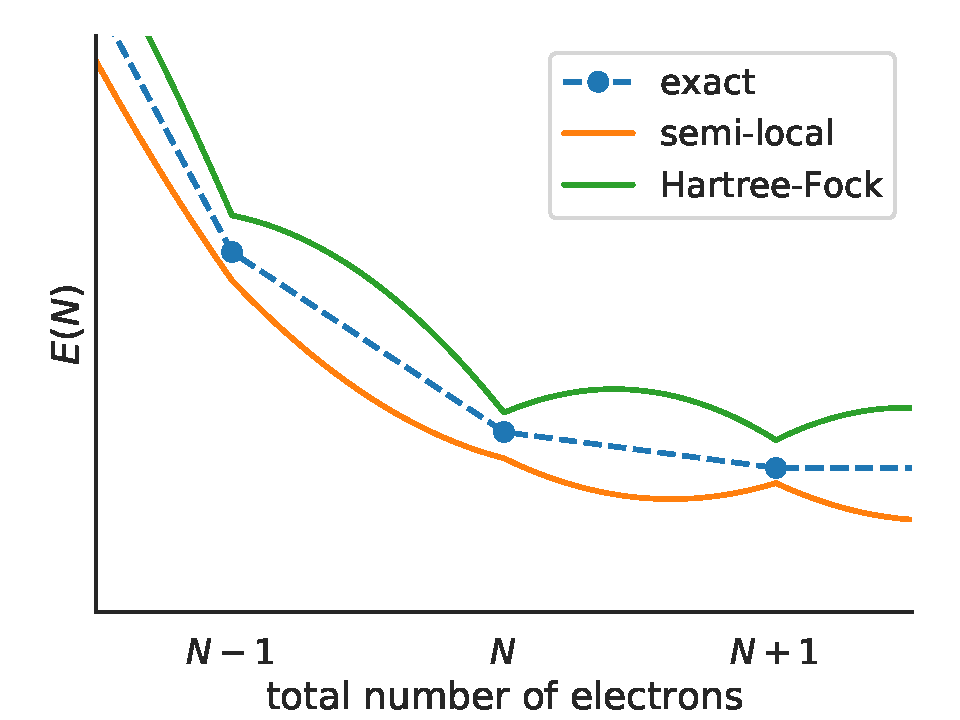
\includegraphics[height=0.7\textheight]{figures/curvature_plot/fig_en_curve_with_all.pdf}
         \end{onlyenv}


         \begin{onlyenv}<2->
            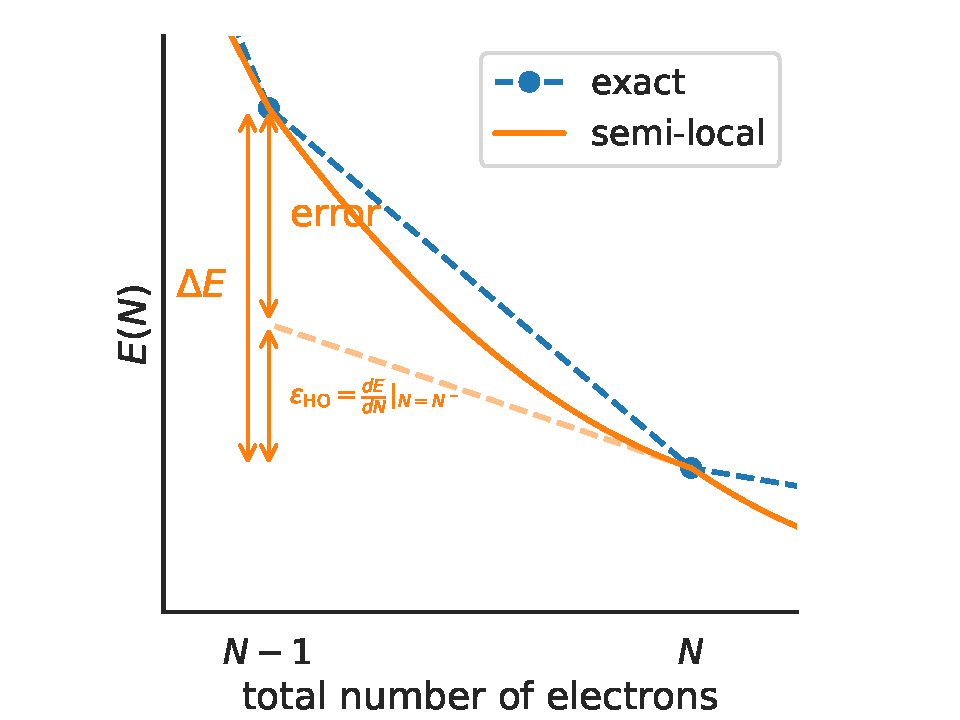
\includegraphics[height=0.7\textheight]{figures/curvature_plot/fig_en_curve_sl_annotated_zoom.pdf}
         \end{onlyenv}
      \end{center}

      \only<3>{\footnotesize Consequences for band gaps, densities, band structures, spectra...}
   \end{overlayarea}

   \blfootcite{Cohen2008,Li2017}

\end{frame}

\begin{frame}{Koopmans spectral functionals: comparing}
   \small
   \renewcommand{\arraystretch}{1.5}
   \rowcolors{1}{seaborn_bg_grey}{seaborn_bg_grey_half}
   \begin{tabularx}{\columnwidth}{L L L}
                                                & \textbf{DFT+\emph{U}}                                                       & \textbf{Koopmans}                                                                                                         \\
      \hline
      designed to correct SIE, as defined by... & erroneous global curvature in total energies                                & dependence of $\varepsilon_i$ on $f_i \ \forall i$ (canonical orbitals)                                                   \\
      by construction...                        & corrects local curvature in total energies                                  & removes dependence of $\varepsilon_i$ on $f_i$ and guarantees $\varepsilon_i = E_i(N\pm 1) - E(N)$ (variational orbitals) \\
      correction applied to...                  & selected subspaces only (e.g. \emph{3d} orbitals)                           & the entire system                                                                                                         \\
      orbitals defined by...                    & Hubbard projectors (atom-centred, frozen, incomplete)                       & variational (minimising) orbitals                                                                                         \\
      corrective parameters are...              & $\{U^I\}$, defined with respect to charge-neutral excitations (if using LR) & $\{\alpha_i\}$, defined with respect to charged excitations                                                               \\
   \end{tabularx}
\end{frame}

\begin{frame}{Outline}
   How can we address self-interaction in a computationally efficient way?

   $\longrightarrow$ Koopmans spectral functionals

   \begin{itemize}
      \item theory
      \item results
      \item outstanding problems
      \item future directions and lessons we can learn
   \end{itemize}

   By way of introduction: DFT+\emph{U}

\end{frame}

\begin{frame}{Koopmans functionals: theory}
   \hbox{
      \begin{minipage}{0.6\textwidth}
         Key idea: construct a functional such that the orbital energies
         \begin{equation*}
            \varepsilon^\mathsf{Koopmans}_i = \braopket{\varphi_i}{H}{\varphi_i} = \partial E_\mathsf{Koopmans}/\partial f_i
         \end{equation*}
         possess two key properties:
         \begin{itemize}
            \item<2-> they are independent of the corresponding occupancies $f_i$ \onslide<3->{($\Leftrightarrow$ $E$ is linear in $f_i$, $\Rightarrow E$ is linear in $N$)}
            \item<4-> they are equal to the corresponding total energy difference $E_i(N-1) - E(N)$ \onslide<5->{$\rightarrow$ orbital energies have meaning, are more accurate}
         \end{itemize}
         %
      \end{minipage}

      \begin{minipage}{0.35\textwidth}
         \centering
         \only<6>{
            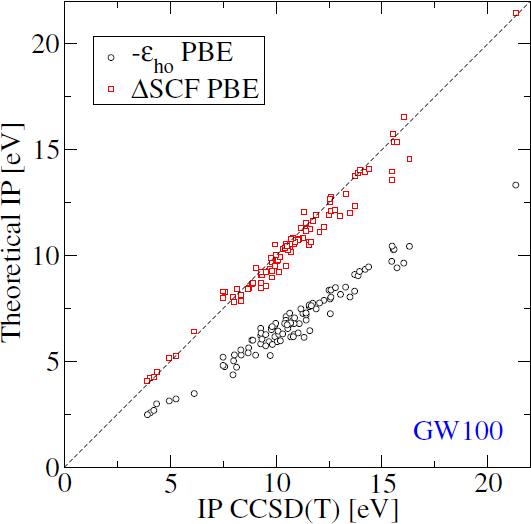
\includegraphics[height=0.6\textheight]{figures/fig_gw100_dscf_cf_ks.png}
         }
      \end{minipage}
   }
\end{frame}
\begin{frame}

   \vspace{1ex}
   \onslide<7->{
      The resulting functional:
      \begin{align*}
          & E_\mathsf{Koopmans} [\rho,
            %\only<7>{\textcolor{red}}
            {\{f_i\}}, {\{\alpha_i\}}]
         = \only<8>{\textcolor{red}}{E_{DFT}[\rho]}
         + \sum_i
         % \only<9->{\textcolor{red}}
         {\alpha_i}
         \left(
         \only<9>{\textcolor{red}}{- \int^{f_i}_{0} \varepsilon_i(f) df}
         \only<10>{\textcolor{red}}{+ f_i \int_0^1 \varepsilon_i(f) df}
         \right)
      \end{align*}
   }
   \begin{minipage}{0.35\textwidth}
      \centering
      \only<6>{
         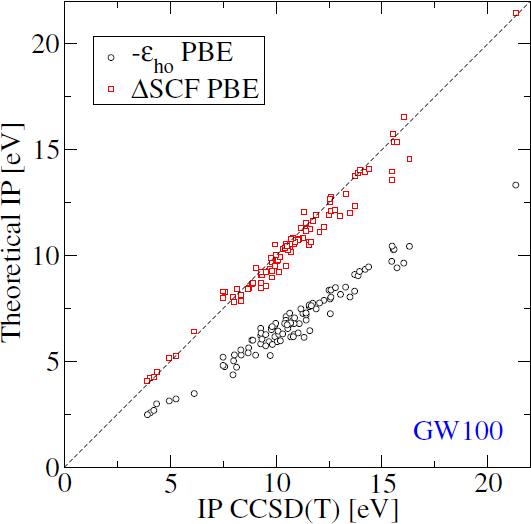
\includegraphics[height=0.6\textheight]{figures/fig_gw100_dscf_cf_ks.png}
      }
      \only<1-5,7>{
         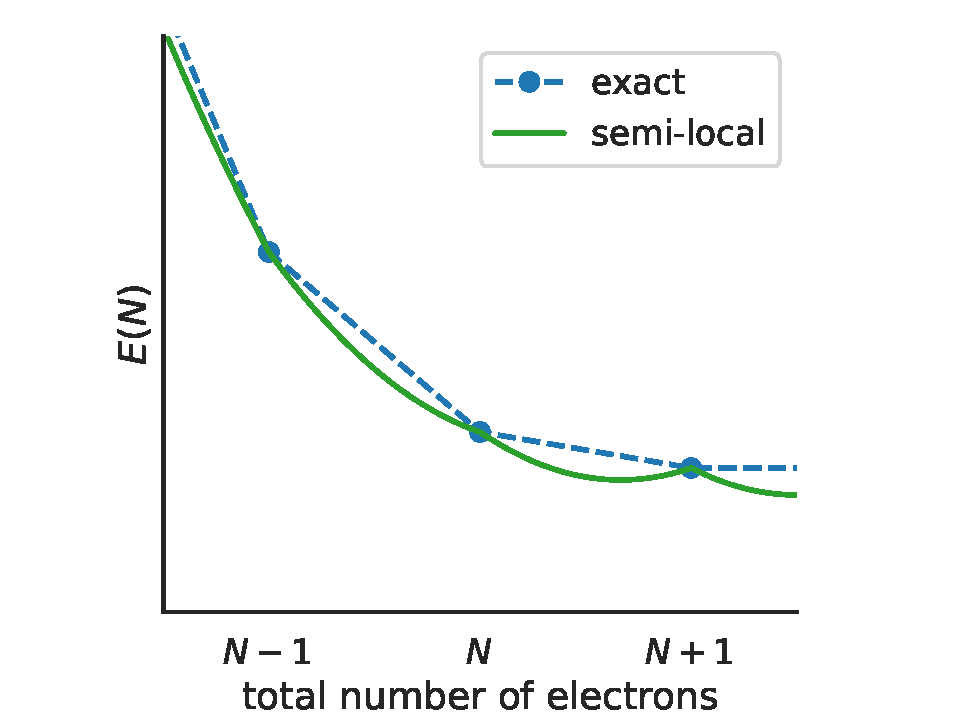
\includegraphics[height=0.6\textheight]{figures/curvature_plot/fig_en_curve_koopmans_step0.pdf}
      }

      \only<8>{
         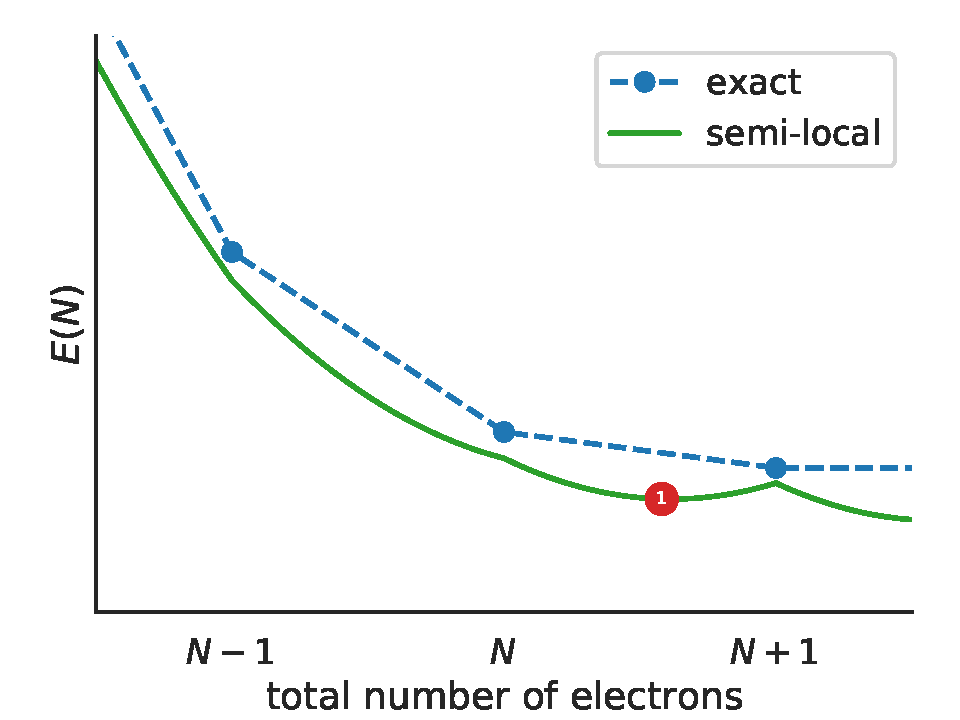
\includegraphics[height=0.6\textheight]{figures/curvature_plot/fig_en_curve_koopmans_step1.pdf}
      }

      \only<9>{
         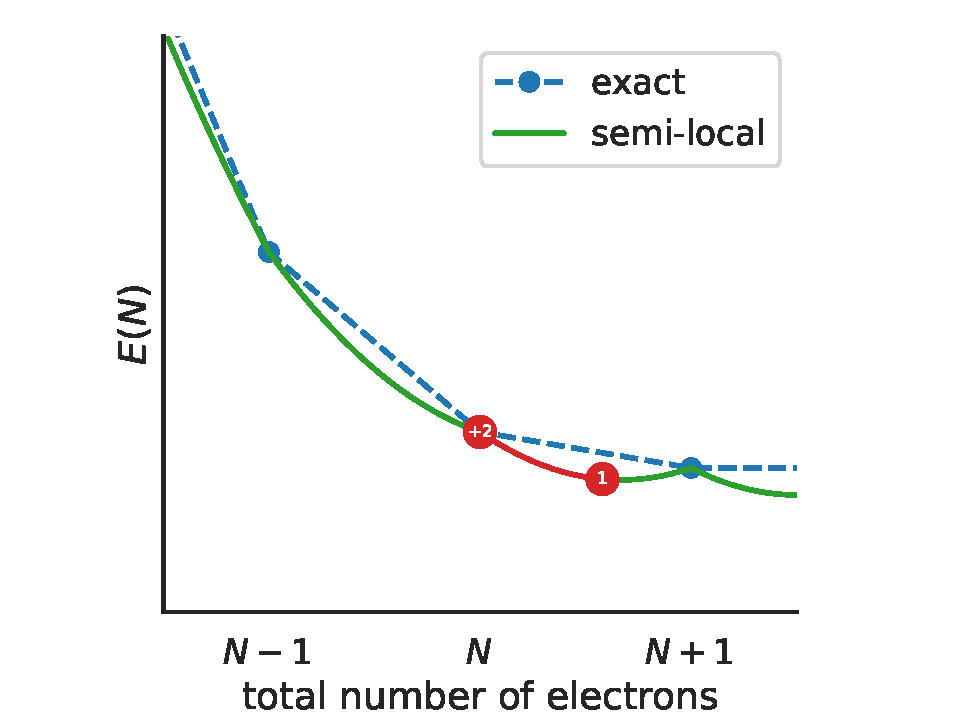
\includegraphics[height=0.6\textheight]{figures/curvature_plot/fig_en_curve_koopmans_step2.pdf}
      }

      \only<10->{
         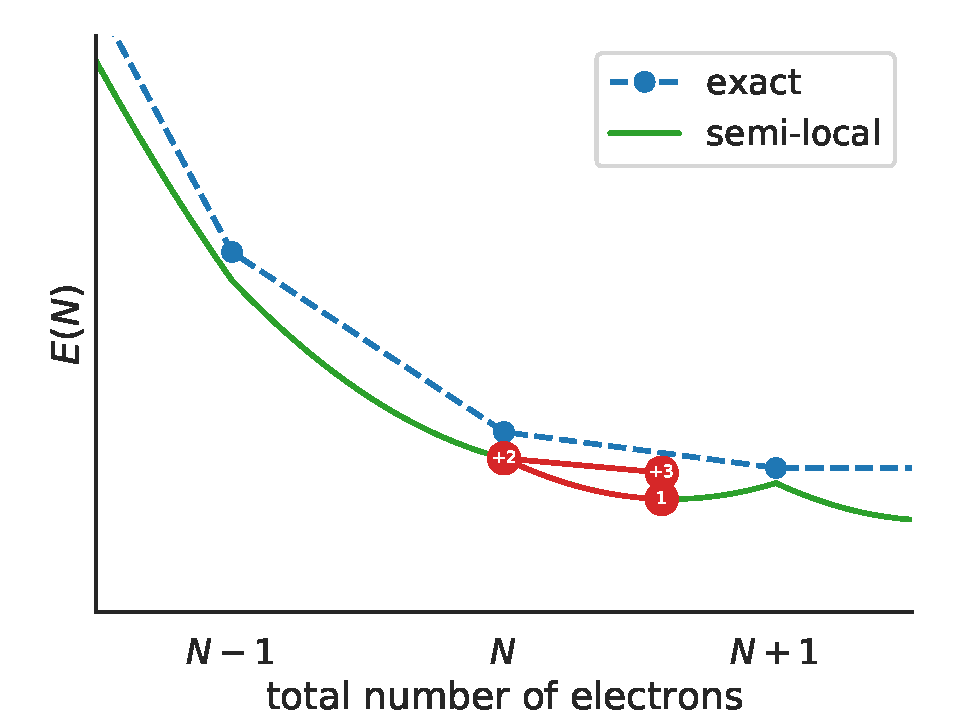
\includegraphics[height=0.6\textheight]{figures/curvature_plot/fig_en_curve_koopmans_step3.pdf}
      }
   \end{minipage}
   % \onslide<10->{
   %    \begin{equation*}
   %       \frac{d E}{d f_i}
   %       \approx
   %       \alpha_i \frac{\partial E}{\partial f_i}
   %       \onslide<11->{
   %          \Longrightarrow \varepsilon_i^\mathsf{Koopmans} = \frac{\partial E_\mathsf{Koopmans}}{\partial f_i}  \approx E_i(N-1) - E(N)}
   %    \end{equation*}
   % }
   \blfootcite{Dabo2010,Borghi2014,Colonna2019}
\end{frame}

\begin{frame}{Koopmans spectral functionals: comparing}
   \small
   \renewcommand{\arraystretch}{1.5}
   \rowcolors{1}{seaborn_bg_grey}{seaborn_bg_grey_half}
   \begin{tabularx}{\columnwidth}{L L L}
                                                & \textbf{DFT+\emph{U}}                                                       & \textbf{Koopmans}                                                                                                           \\
      \hline
      designed to correct SIE, as defined by... & erroneous global curvature in total energies                                & \leavevmode\onslide<2->{dependence of $\varepsilon_i$ on $f_i \ \forall i$}                                                 \\
      by construction...                        & corrects local curvature in total energies                                  & \leavevmode\onslide<3->{removes dependence of $\varepsilon_i$ on $f_i$ and guarantees $\varepsilon_i = E_i(N\pm 1) - E(N)$} \\
      correction applied to...                  & selected subspaces only (e.g. \emph{3d} orbitals)                           & \leavevmode\onslide<4->{the entire system}                                                                                  \\
      orbitals defined by...                    & Hubbard projectors (atom-centred, frozen, incomplete)                       &                                                                                                                             \\
      corrective parameters are...              & $\{U^I\}$, defined with respect to charge-neutral excitations (if using LR) &
   \end{tabularx}
\end{frame}

\begin{frame}{Koopmans spectral functionals: theory}
   \begin{equation*}
      E_\mathsf{Koopmans}[\rho,\only<2-3>{\textcolor{red}}{\{f_i\}}, \only<5->{\textcolor{red}}{\{\alpha_i\}}] = E_{DFT}[\rho]
      + \sum_i
      \only<5->{\textcolor{red}}
      {\alpha_i}
      \left(
      - \int^{f_i}_{0} \varepsilon_i(f) df
      + f_i \int_0^1 {\varepsilon_i(f)} df
      \right)
   \end{equation*}

   \onslide<3->{
      \begin{equation*}
         v^\mathrm{KI}_i/\alpha_i = - E_{\mathrm{H}}\left[n_{i}\right]
         + E_{\mathrm{xc}}\left[\rho\right]
         - E_{\mathrm{xc}}\left[\rho-n_{i}\right]
         - \int d\mathbf{r'}
         v_\mathrm{xc}(\mathbf{r}', [\rho])
         n_{i}(\mathbf{r}')
      \end{equation*}
   }

   \vspace{-1ex}
   \begin{itemize}
      \item<2-> orbital density dependence
      \item<4-> variational (localised, minimising) vs canonical (delocalised, diagonalising) orbitals
      \item<5-> screening
   \end{itemize}
   \begin{overlayarea}{\textwidth}{0.4\textheight}
      \only<4>{
         \begin{figure}[t]
            \centering
            \begin{subfigure}{0.3\textwidth}
               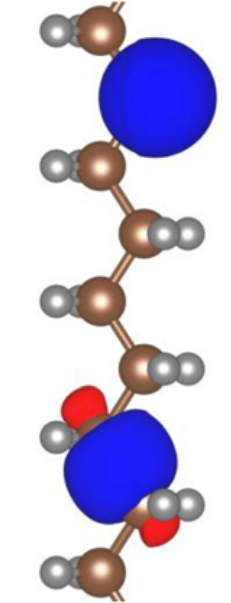
\includegraphics[height=\columnwidth,angle=90]{figures/fig_nguyen_variational_orbital.png}
               \caption{variational}
            \end{subfigure}
            \hspace{0.1\textwidth}
            \begin{subfigure}{0.3\textwidth}
               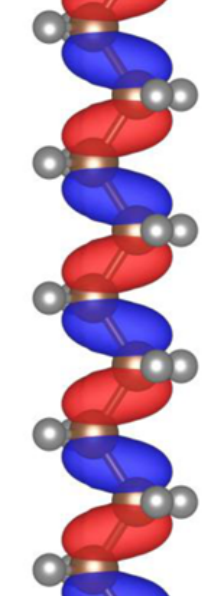
\includegraphics[height=\columnwidth,angle=90]{figures/fig_nguyen_canonical_orbital.png}
               \caption{canonical}
            \end{subfigure}
         \end{figure}
      }
      \only<5->{
         \begin{equation*}
            \frac{d E}{d f_i}
            \approx
            \alpha_i \frac{\partial E}{\partial f_i}
            \onslide<6->{
               \Longrightarrow \varepsilon_i^\mathsf{Koopmans} = \frac{\partial E_\mathsf{Koopmans}}{\partial f_i}  \approx E_i(N-1) - E(N)}
         \end{equation*}
      }
   \end{overlayarea}
   \blfootcite{Nguyen2018}
\end{frame}

\begin{frame}{Koopmans spectral functionals: comparing}
   \small
   \renewcommand{\arraystretch}{1.5}
   \rowcolors{1}{seaborn_bg_grey}{seaborn_bg_grey_half}
   \begin{tabularx}{\columnwidth}{L L L}
                                                & \textbf{DFT+\emph{U}}                                                       & \textbf{Koopmans}                                                                                                                                                   \\
      \hline
      designed to correct SIE, as defined by... & erroneous global curvature in total energies                                & dependence of $\varepsilon_i$ on $f_i \ \forall i$ \leavevmode\onslide<4->{\textcolor{red}{(canonical orbitals)}}                                                   \\
      by construction...                        & corrects local curvature in total energies                                  & removes dependence of $\varepsilon_i$ on $f_i$ and guarantees $\varepsilon_i = E_i(N\pm 1) - E(N)$ \leavevmode\onslide<4->{\textcolor{red}{(variational orbitals)}} \\
      correction applied to...                  & selected subspaces only (e.g. \emph{3d} orbitals)                           & the entire system                                                                                                                                                   \\
      orbitals defined by...                    & Hubbard projectors (atom-centred, frozen, incomplete)                       & \leavevmode\onslide<2->{variational (minimising) orbitals}                                                                                                          \\
      corrective parameters are...              & $\{U^I\}$, defined with respect to charge-neutral excitations (if using LR) & \leavevmode\onslide<3->{$\{\alpha_i\}$, defined with respect to charged excitations}                                                                                \\
   \end{tabularx}
\end{frame}

\begin{frame}{Koopmans spectral functionals: IPs}
   Ionisation potentials $ = E(N-1) - E(N) \stackrel{?}{=} -\varepsilon_{HO}$ of 100 molecules (the GW100 set) cf. CCSD(T)
   \begin{center}
      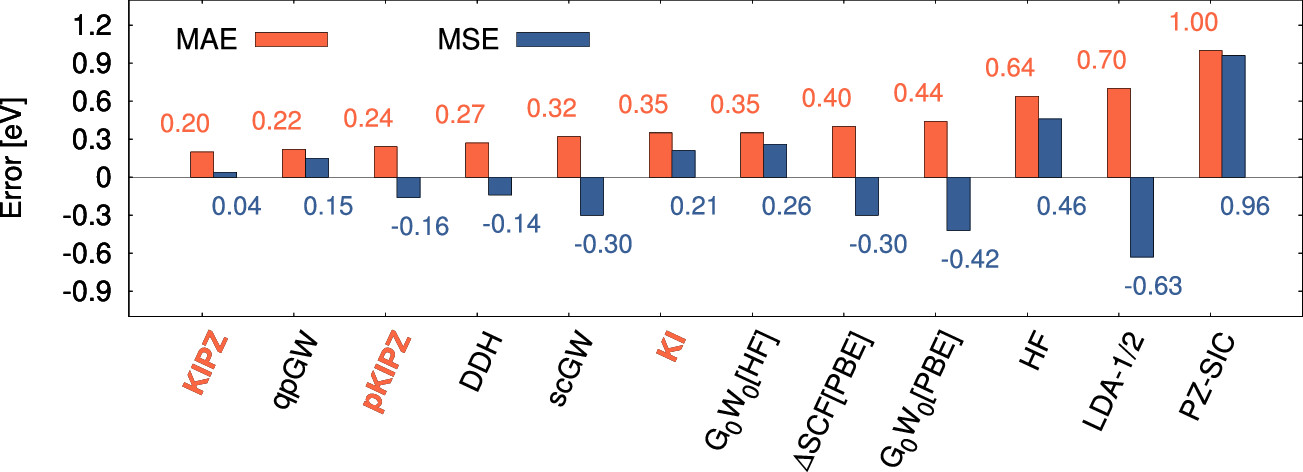
\includegraphics[height=0.23\textwidth]{figures/colonna_2019_gw100_ip}
      \onslide<2->{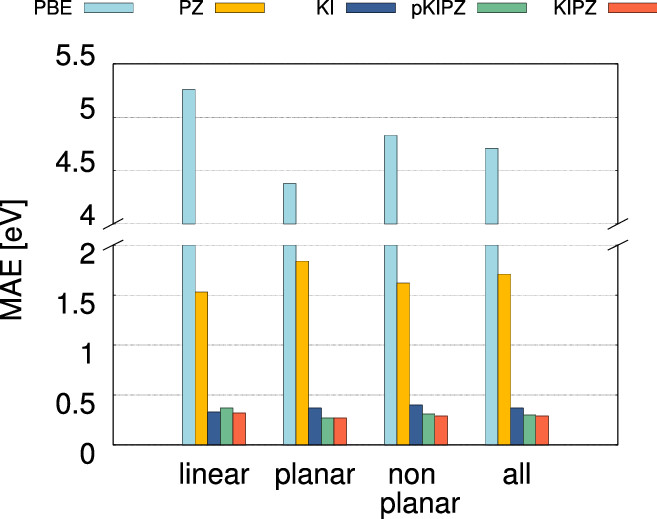
\includegraphics[height=0.23\textwidth]{figures/colonna_2019_gw100_deeper}}
   \end{center}

   \blfootcite{Colonna2018,vanSetten2015}
\end{frame}

\begin{frame}{Koopmans spectral functionals: EAs}
   Electron affinities $ = E(N) - E(N+1) \stackrel{?}{=} -\varepsilon_{LU}$ of molecules cf. CCSD(T)/exp
   \vspace{2ex}

   \small
   \begin{center}
      \begin{tabular}{c c}
         For 15 of the GW100 molecules with bound LUMOs                            &
         For the NaCl molecule                                                       \\
         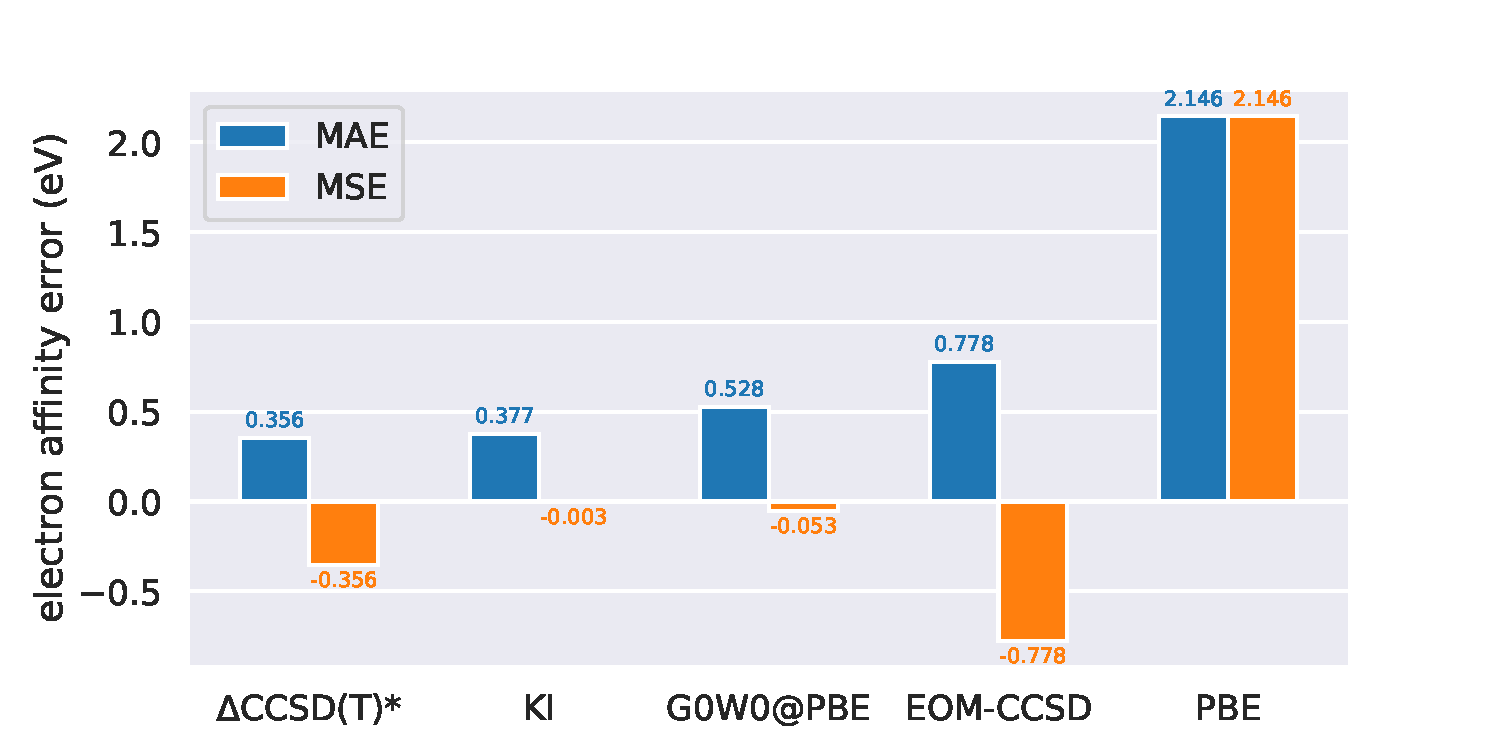
\includegraphics[height=0.5\textheight]{figures/fig_gw100_ea_mae_mse.pdf} &
         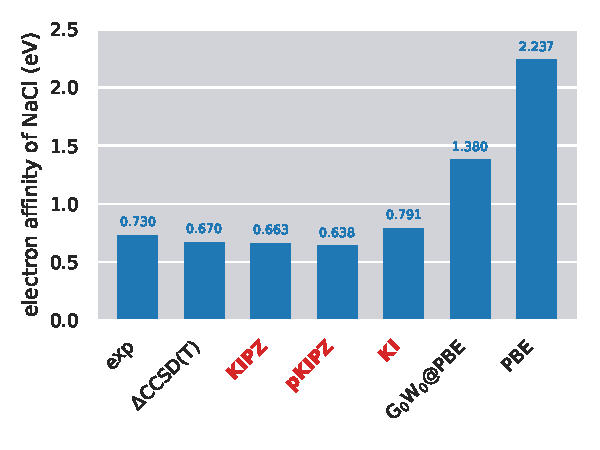
\includegraphics[height=0.5\textheight]{figures/fig_NaCl_eas.pdf}           \\
      \end{tabular}
      \textcolor{seaborn_bg_grey_darker}{Figures from Linscott et al. (in prep)}
   \end{center}


\end{frame}


\begin{frame}{Koopmans spectral functionals: spectra}
   \begin{center}
      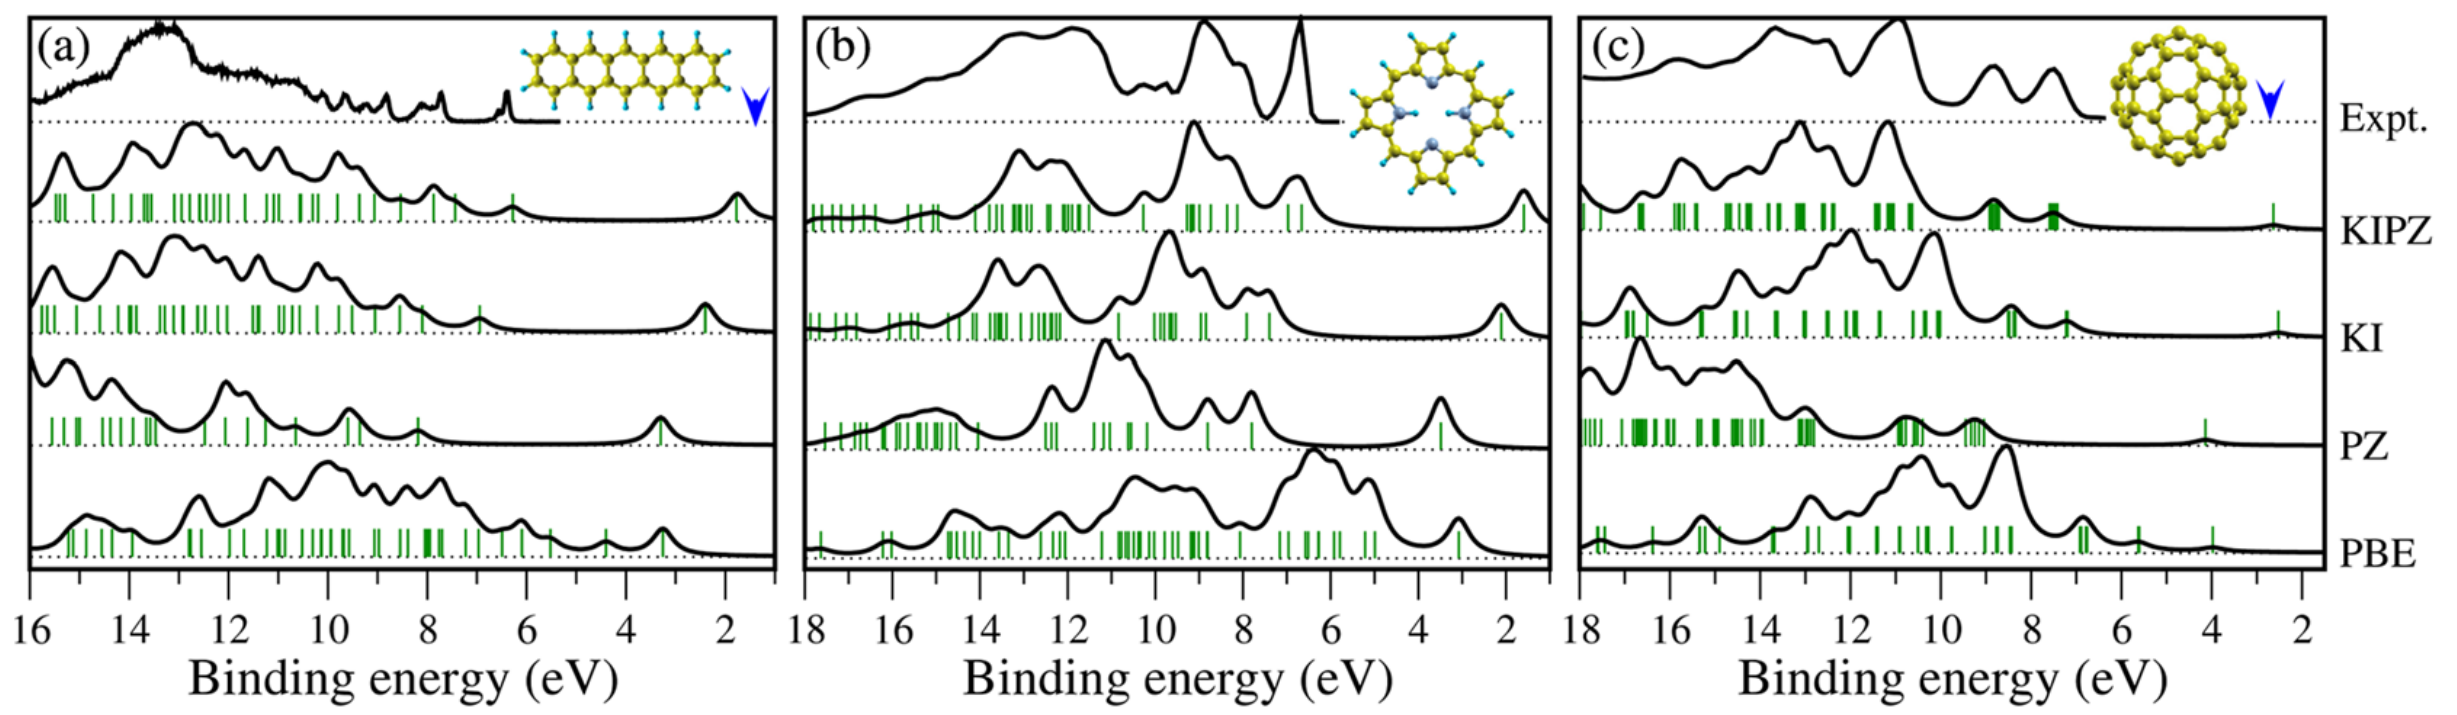
\includegraphics[height=0.5\textheight]{figures/fig_nguyen_prl_spectra.png}
   \end{center}
   \blfootcite{Nguyen2015}
\end{frame}

\begin{frame}{\normalsize Koopmans spectral functionals: band structures}
   \begin{figure}[t]
      \centering
      \begin{subfigure}{0.45\textwidth}
         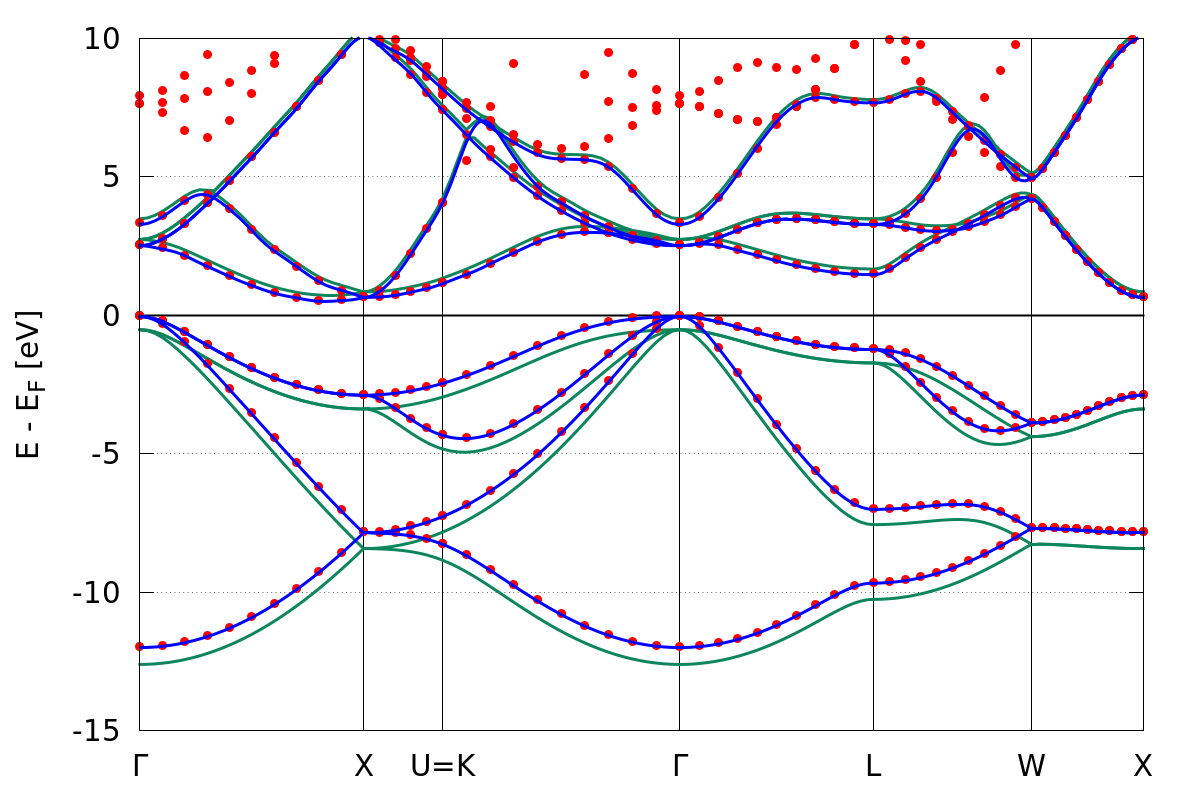
\includegraphics[width=\columnwidth]{figures/Si_kipz_bands.png}
         \caption{Si, KIPZ}
         \footnotesize
         \begin{tabularx}{\columnwidth}{l C C C C}
                                  & PBE  & qsGW & KIPZ & exp. \\
            \hline
            $E_\mathrm{gap}$ (eV) & 0.55 & 1.30 & 1.27 & 1.22 \\
            \vphantom{Test}
         \end{tabularx}
      \end{subfigure}
      \begin{subfigure}{0.45\textwidth}
         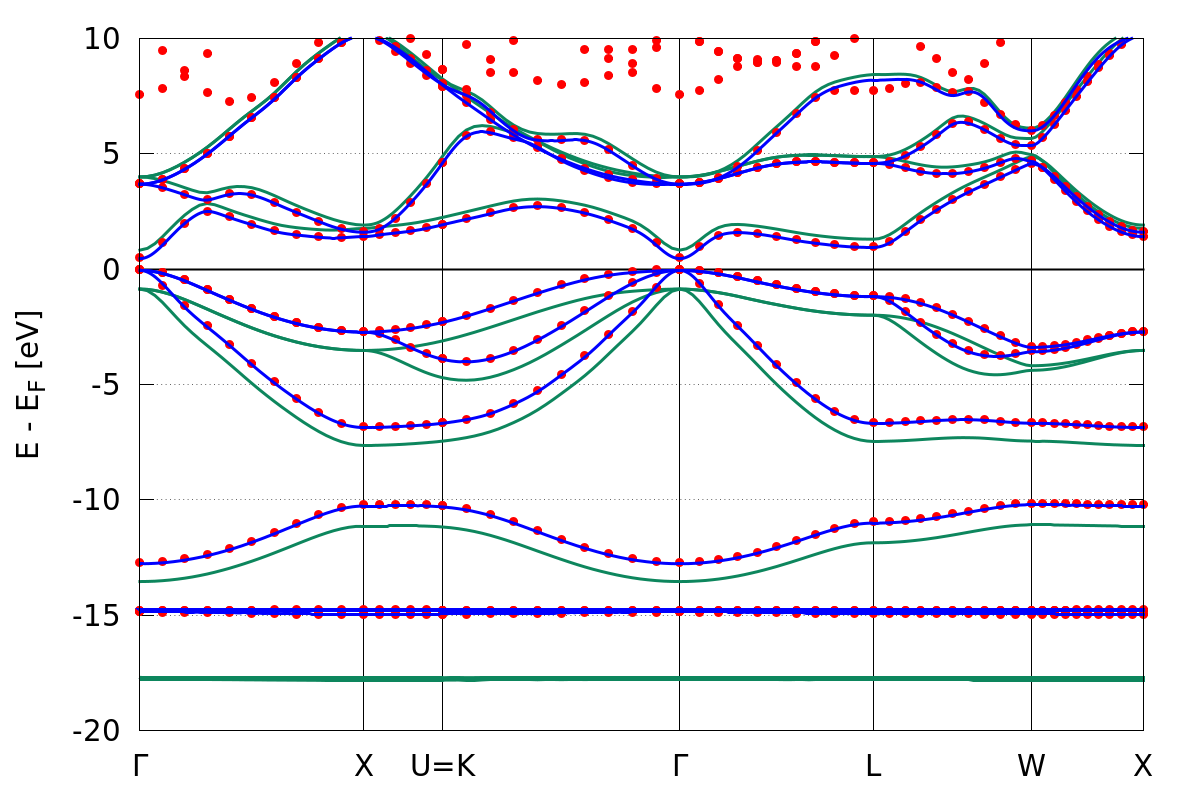
\includegraphics[width=\columnwidth]{figures/GaAs_ki_bands.png}
         \caption{GaAs, KI}
         \footnotesize
         \begin{tabularx}{\columnwidth}{l C C C C}
                                                 & PBE   & qsGW & KI    & exp.  \\
            \hline
            $E_\mathrm{gap}$ (eV)                & 0.50  & 1.51 & 1.68  & 1.57  \\
            $\langle \varepsilon_d \rangle$ (eV) & -14.9 &      & -17.0 & -18.9
         \end{tabularx}
      \end{subfigure}
      % \begin{subfigure}{\textwidth}
      %    \begin{tabularx}{\columnwidth}{C C C C C C C}
      %       ZnO                                  & LDA  & HSE  & GW$_0$ & scG$\tilde{\rm W}$ & KI   & exp.      \\
      %       \hline
      %       $E_\mathrm{gap}$ (eV)                & 0.79 & 2.79 & 3.0    & 3.2                & 3.62 & 3.60      \\
      %       $\langle \varepsilon_d \rangle$ (eV) & -5.1 & -6.1 & -6.4   & -6.7               & -6.9 & -7.5/-8.0 \\
      %    \end{tabularx}
      % \end{subfigure}
   \end{figure}
   \blfootcite{DeGennaro2021}
\end{frame}

\begin{frame}{\normalsize Koopmans spectral functionals: band structures}
   \begin{figure}[t]
      \centering
      \begin{subfigure}{0.3\textwidth}
         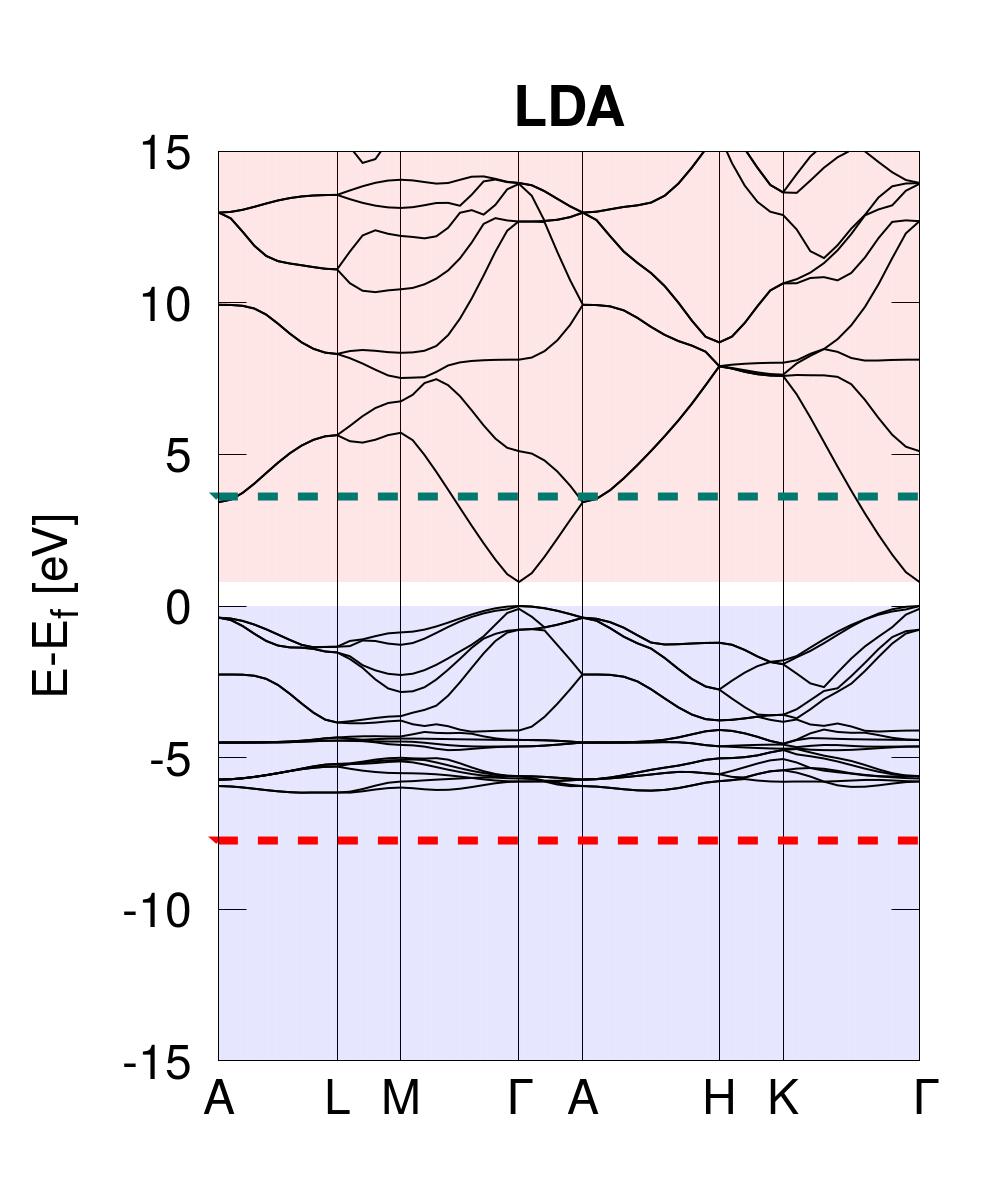
\includegraphics[width=\columnwidth]{figures/ZnO_lda.png}
      \end{subfigure}
      \begin{subfigure}{0.3\textwidth}
         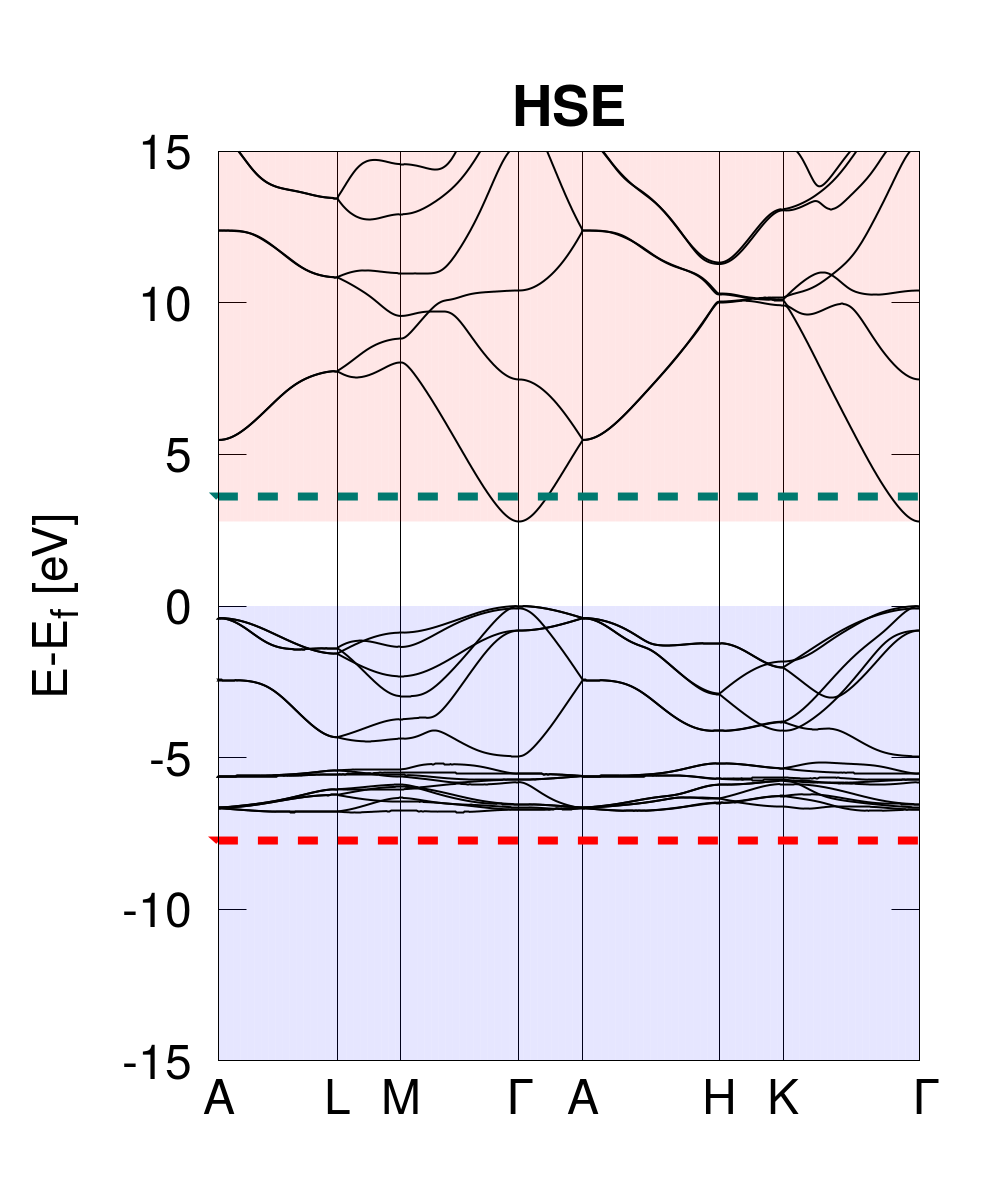
\includegraphics[width=\columnwidth]{figures/ZnO_hse.png}
      \end{subfigure}
      \begin{subfigure}{0.3\textwidth}
         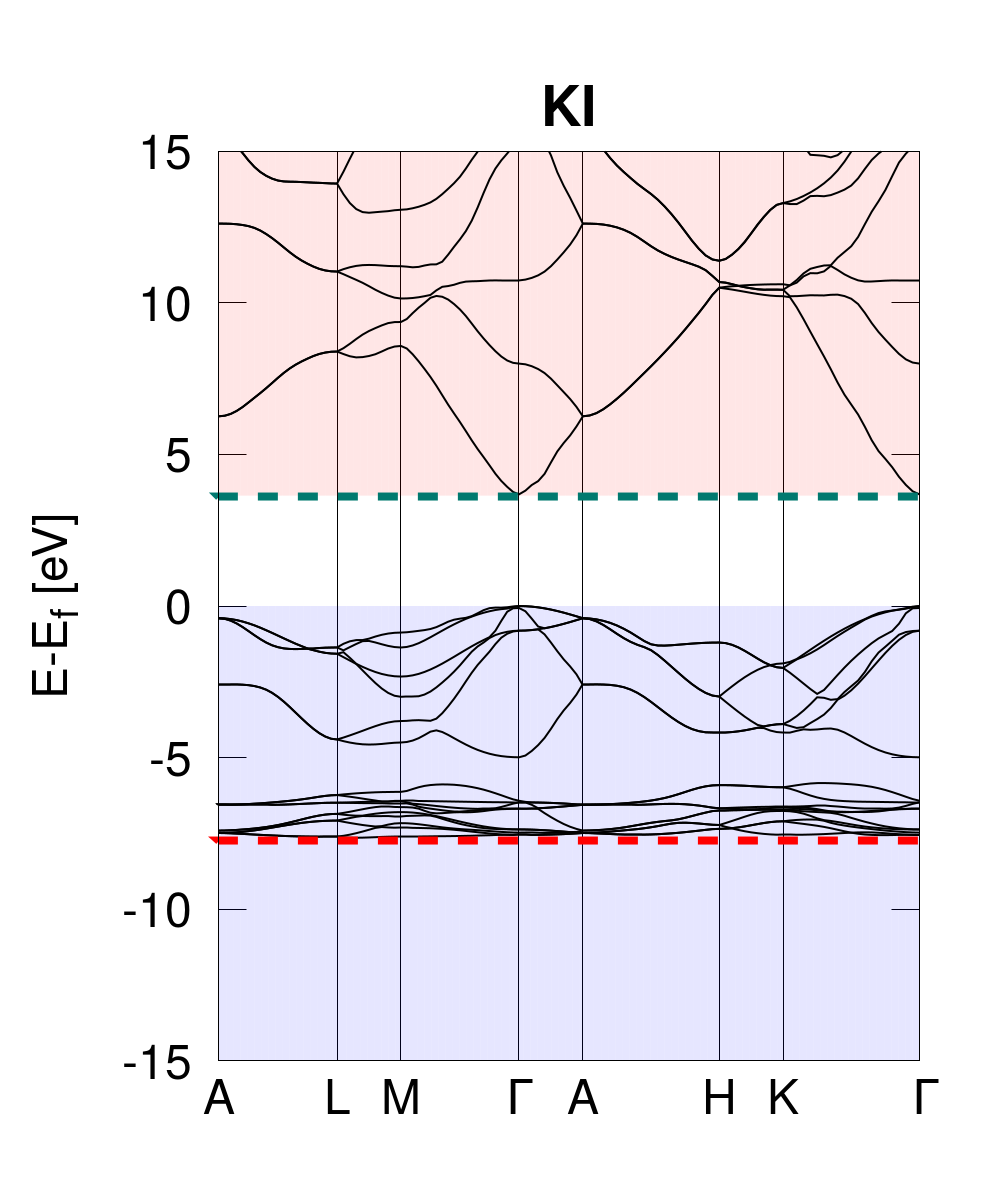
\includegraphics[width=\columnwidth]{figures/ZnO_ki.png}
      \end{subfigure}
      \begin{subfigure}{\textwidth} %<-- changed width
         %        \centering
         %    \renewcommand\tabularxcolumn[1]{m{#1}}% <-- added
         %    \renewcommand\arraystretch{1.3}
         %    \setlength\tabcolsep{2pt}% <-- added
         \begin{tabularx}{\columnwidth}{C C C C C C C}
            ZnO                                  & LDA  & HSE  & GW$_0$ & scG$\tilde{\rm W}$ & KI   & exp.      \\
            \hline
            $E_\mathrm{gap}$ (eV)                & 0.79 & 2.79 & 3.0    & 3.2                & 3.62 & 3.60      \\
            $\langle \varepsilon_d \rangle$ (eV) & -5.1 & -6.1 & -6.4   & -6.7               & -6.9 & -7.5/-8.0 \\
         \end{tabularx}
         %        \caption{table}
      \end{subfigure}
      % \caption{Band structure of ZnO calculated at different level of theory:
      %    LDA (left panel), HSE (middle panel) and KI (right panel). Shaded areas
      %    highlight valence (light blue) and conduction (light red) manifolds. The
      %    experimental values for the band gap and for the energy position of
      %    Zn $d$-states are represented by the dashed green line and by the dashed
      %    red line, respectively.
      %    Table: Band gap and position of Zn $d$ states with respect to the top of the valence band at different level of theory compared to experimental and GW results from Ref.~\onlinecite{shishkin_accurate_2007}.}
   \end{figure}
   \blfootcite{Colonna2021}
\end{frame}

\begin{frame}{\small Koopmans spectral functionals: practical limitations}
   \begin{itemize}
      \item determining $\{\alpha_i\}$
      \item how to treat metals?
      \item limitations of the orbital-density-dependent framework
   \end{itemize}
\end{frame}


\begin{frame}{\small Koopmans spectral functionals: the workflow(s)}
   \small Screening coefficients $\{\alpha_i\}$ must be determined first, either \onslide<2->{(a) via $\Delta$SCF calculations (using a supercell) or} \onslide<4->{(b) via DFPT\footcite{Colonna2018} (using a primitive cell)}
   \vspace{1ex}

   \onslide<3->{
      Supercell implementation

      \vspace{-2ex}
      \adjustbox{width=\textwidth}{\begin{tikzpicture}[font=\tiny, x=3.5cm, y=1cm]
\begin{pgfonlayer}{background}
   % \node[fit= (KC init) (empty label) (filled label) (sc loop 1) (converged label), fill=seaborn_bg_grey, inner sep=0.5cm] (calculating screening) {};
   % \node [dummy, above=0cm of calculating screening, font=\sffamily]{Calculating screening parameters};
   \fill [seaborn_bg_grey_dark] (-2.1,-0.8) rectangle (1.3,4.6);
   \node at (-2.1, 4.6) [default_text] {\large Initialisation (molecules)};
   \fill [seaborn_bg_grey_dark] (-2.1,-4.6) rectangle (1.3,-1.2);
   \node at (-2.1, -1.2) [default_text] {\large Initialisation (solids)};
   \fill [seaborn_bg_grey_dark] (1.4,-4.6) rectangle (6.9,4.6);
   \node at (1.4, 4.6) [default_text] {\large Calculating screening parameters};
   \fill [seaborn_bg_grey_dark] (7,-4.6) rectangle (8,4.6);
   \node at (7, 4.6) [default_text, text width=3.5cm] {\large Final calculation};
   \fill [seaborn_bg_grey_dark] (8.1,-4.6) rectangle (9.1,4.6);
   \node at (8.1, 4.6) [default_text, text width=3.5cm] {\large Postprocessing (solids)};
\end{pgfonlayer}

% Key
\node at (6.85, 5.25) [cp, text width=1.4cm, minimum height=0.7cm] {\texttt{cp}};
\node at (7.35, 5.25) [pw, text width=1.4cm, minimum height=0.7cm] {\texttt{pw}};
\node at (7.85, 5.25) [wannier90, text width=1.4cm, minimum height=0.7cm] {\texttt{wannier90}};
\node at (8.35, 5.25) [bespoke, text width=1.4cm, minimum height=0.7cm, font=\tiny] {bespoke code};
\node at (8.85, 5.25) [observable, text width=1.4cm, minimum height=0.7cm, font=\tiny] {quantity of interest};

% Initialisation
% Option 1
\node at (-1, 2.9) [cp] (PBE init) {PBE};
\node at (0, 2.9) [cp] (PZ innerloop) {PZ unitary rotation};
\path [line] (PBE init) -- (PZ innerloop);

% OR
\node at (-0.5, 1.9) [default] (or) {or};

% Option 2
\node at (-0.5, 0.9) [cp] (PZ init) {PZ};

% Solids
\node at (-1.5, -2.9) [pw] (pw PBE init) {PBE (primitive cell)};
\node at (-0.5, -2.9) [wannier90] (wannierize) {wannierize};
\node at (0.5, -2.9) [bespoke] (unfold) {fold to supercell};
\path [line] (pw PBE init) -- (wannierize);
\path [line] (wannierize) -- (unfold);

% Calculating screening parameters
\node at (2, 0) [cp] (KC init) {$\alpha_0$KI/$\alpha_0$KIPZ};

\path let
\p1 = (PZ innerloop),
\p2 = (unfold.east)
in
coordinate (dummy) at (\x2, \y1);
\path let
\p1 = (PZ init),
\p2 = (unfold.east)
in
coordinate (dummy2) at (\x2, \y1);
\path [line] (PZ innerloop) -- (dummy) to[-|-=0.3] ([yshift=2\myyshift]KC init.west);
\path [line] (PZ init.east) -- ([xshift=-3.5\myyshift]dummy2) to[-|-=0.3] (KC init.west);
\path [line] ([yshift=-2\myyshift]unfold.east) to[-|-=0.3] ([yshift=-2\myyshift]KC init.west);

% KI filled %%%%%%%%%%%%%%%%%%%%%%%%%%%%%%%%%%%%%%%%%%%%%%%%%%

% calculations
\node at (3, 3) [cp] (N-1_filled) {PBE/$\alpha_0$KIPZ ($N-1$)};
\node at (3, 2) [cp] (PBE_filled) {PBE};
\node at (3, -2) [cp] (PBE_empty) {PBE};
\node at (3, -3) [cp] (N+1_empty) {PBE/$\alpha_0$KIPZ ($N+1$)};

\path [line] (KC init) to[-|-] (PBE_filled);
\path [line] (KC init) to[-|-] (N-1_filled);
\path [line] (KC init) to[-|-] (PBE_empty);
\path [line] (KC init) to[-|-] (N+1_empty);

% results
\node at (4, 3) [observable] (EN-1_filled) {$E_i(N-1)$};
\node at (4, 2) [observable] (lambda0_filled) {$\lambda^{0}_{ii}(1)$};
\node at (4, 1) [observable] (lambda_filled) {$\lambda^{\alpha_0}_{ii}(1)$};
\node at (4, 0) [observable] (EN) {$E(N)$};
\node at (4, -1) [observable] (lambda_empty) {$\lambda^{\alpha_0}_{ii}(0)$};
\node at (4, -2) [observable] (lambda0_empty) {$\lambda^{0}_{ii}(0)$};
\node at (4, -3) [observable] (EN+1_empty) {$E_i(N+1)$};

\path [line] (KC init) -- (EN);
\path [line] (KC init.east) to[-|-] (lambda_filled.west);
\path [line] (KC init.east) to[-|-] (lambda_empty.west);

\path [line] (PBE_filled) -- (lambda0_filled);
\path [line] (N-1_filled) -- (EN-1_filled);

\path [line] (PBE_empty) -- (lambda0_empty);
\path [line] (N+1_empty) -- (EN+1_empty);

% alpha parameters
\node at (5, 1.5) [observable] (alpha filled) {$\alpha_{i \in \text{filled}}$};
\node at (5, -1.5) [observable] (alpha empty) {$\alpha_{i \in \text{empty}}$};

\path [line] (lambda_filled) to[-|-] (alpha filled);
\path [line] ([yshift=\myyshift]EN.east) to[-|-] (alpha filled.west);
\path [line] (lambda0_filled) to[-|-] (alpha filled);
\path [line] (EN-1_filled) to[-|-] (alpha filled);

\path [line] (lambda_empty) to[-|-] (alpha empty);
\path [line] ([yshift=-\myyshift]EN.east) to[-|-] (alpha empty.west);
\path [line] (lambda0_empty) to[-|-] (alpha empty);
\path [line] (EN+1_empty) to[-|-] (alpha empty);

% SC check
\coordinate (sc check) at (6, 0);
\path [headless_line] (alpha empty) to[-|-] (sc check);
\path [headless_line] (alpha filled) to[-|-] (sc check);

% SC loop
\node [below= of EN+1_empty] (sc loop y) {};
\path let
\p1 = (sc check),
\p2 = (sc loop y)
in
coordinate (sc loop 1) at (\x1, \y2);
\path [line] (sc check) -- node [midway, right, font=\sffamily] (not converged label) {\footnotesize $\{\alpha_i\}$ not converged} (sc loop 1) -| (KC init.south);

% Final calc
\node at (7.5, 0) [cp] (final KI) {$\alpha$KI/$\alpha$KIPZ};
\path [line] (sc check) -- node [midway, above, font=\sffamily] (converged label) {\footnotesize $\{\alpha_i\}$ converged} (final KI);

% Postproc
\node at (8.6, 0) [bespoke] (upfold) {unfold to primitive cell};
\path [line] (final KI) -- (upfold);

% Boxes
% Screening parametere
\node [boxwhite, fit= (N-1_filled) (lambda_filled) (alpha filled),
   draw, dashed, fill opacity=0, inner sep=0.35cm](filled box){};
\node [dummy, above=0cm of filled box, font=\sffamily](filled label){one per filled orbital (index $i$)};
\node [boxwhite, fit= (N+1_empty) (lambda_empty) (alpha empty),
   draw, dashed, fill opacity=0, inner sep=0.35cm](empty box){};
\node [dummy, below=0cm of empty box, font=\sffamily](empty label){one per empty orbital (index $i$)};

% \onslide<2->{
%    \node at (3.5, 0) [default_text, fill=white, opacity=0.9, text opacity=1, anchor=center, minimum height=5cm, text width=7.5cm, execute at begin node=\setlength{\baselineskip}{30pt}] (nc text) {
%       \huge Riccardo De Gennaro
%       \textbf{M22.00004} / paper in preparation
%    };
%    \node[right = -0.2cm of nc text, anchor=west]{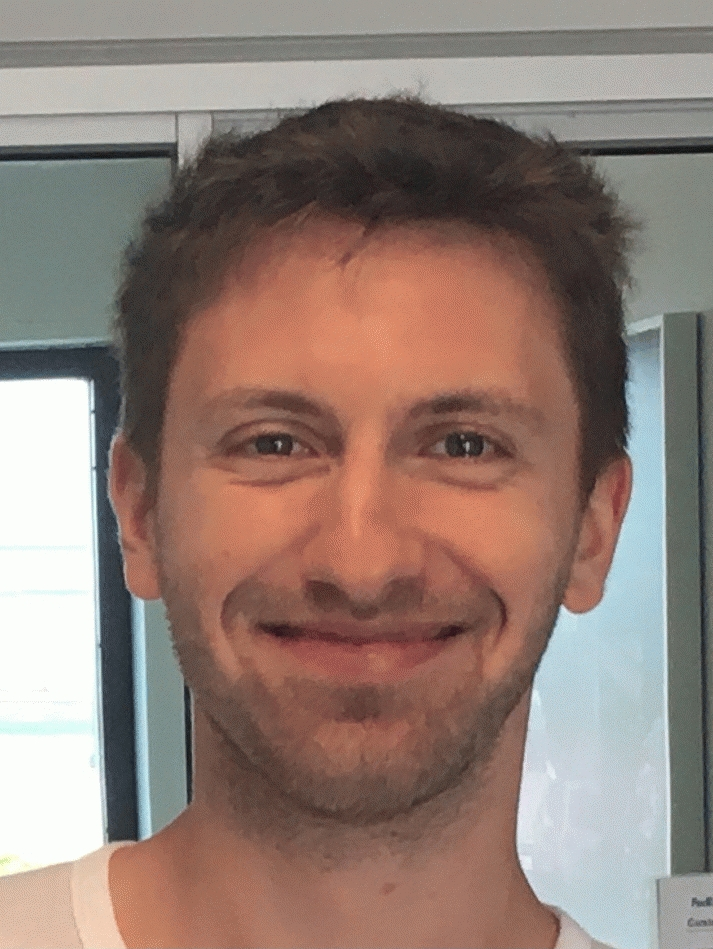
\includegraphics[height=5cm]{figures/riccardo_degennaro.jpg}};
% }


% ML
}
   }

   \vspace{-1.5ex}
   \onslide<5->{
      \noindent Primitive cell implementation

      \vspace{-2ex}
      \adjustbox{width=0.655\textwidth}{\begin{tikzpicture}[font=\tiny, x=3.5cm, y=1cm]
   \begin{pgfonlayer}{background}
      \fill [seaborn_bg_grey_dark] (-2.2,-1) rectangle (1.2,1.5);
      \node at (-2.2, 1.5) [default_text] {\large Initialisation};
      \fill [seaborn_bg_grey_dark] (1.3,-1) rectangle (3.7,1.5);
      \node at (1.3, 1.5) [default_text] {\large Calculating screening parameters};
      \fill [seaborn_bg_grey_dark] (3.8,-1) rectangle (5.2,1.5);
      \node at (3.8, 1.5) [default_text, text width=3.5cm] {\large Final calculation};
      % \fill [seaborn_bg_grey_dark] (8.1,-1) rectangle (9.1,1.5);
      % \node at (8.1, 1.5) [default_text, text width=3.5cm] {\large Postprocessing};
   \end{pgfonlayer}

   % Key
   \node at (3.45, 2.15) [pw, text width=1.4cm, minimum height=0.7cm] {\texttt{pw}};
   \node at (3.95, 2.15) [wannier90, text width=1.4cm, minimum height=0.7cm] {\texttt{wannier90}};
   \node at (4.45, 2.15) [bespoke, text width=1.4cm, minimum height=0.7cm, font=\tiny] {bespoke code};
   \node at (4.95, 2.15) [observable, text width=1.4cm, minimum height=0.7cm, font=\tiny] {quantity of interest};

   % Initialisation
   % Solids
   \node at (-1.5, 0) [pw] (pw PBE init) {PBE};
   \node at (-0.5, 0) [wannier90] (wannierize) {wannierize};
   \node at (0.5, 0) [observable] (unfold) {$\{\ket{w_i}\}$};
   \path [line] (pw PBE init) -- (wannierize);
   \path [line] (wannierize) -- (unfold);

   % Calculating screening parameters
   \node at (2, 0) [bespoke] (KC screen) {DFPT calculation};
   \node at (3, 0) [observable] (alphas) {$\{\alpha_i\}$};
   \path [line] (unfold) -- (KC screen);
   \path [line] (KC screen) -- (alphas);

   % Final calc
   \node at (4.5, 0) [bespoke] (KC ham) {$\alpha_0$KI/$\alpha_0$KIPZ};
   \path [line] (alphas) -- (KC ham);

   % \onslide<4->{
   %    \node at (1, 0) [default_text, fill=white, opacity=0.9, text opacity=1, anchor=center, minimum height=5cm, text width=7cm, execute at begin node=\setlength{\baselineskip}{30pt}] (nc text) {
   %       \huge Nicola Colonna
   %       \textbf{A20.00002} /
   %       paper in preparation
   %    };
   %    \node[right = -0.2cm of nc text, anchor=west]{
\includegraphics[height=5cm]{figures/nicola_colonna.png}};
   % }
    \onslide<4->{
      \fill [seaborn_bg_grey_dark,opacity=0.8] (1.3,-1) rectangle (3.7,1.5);
      \node at (2.5, 0) [cp, fill=seaborn_yellow, font=\Huge, inner sep=10pt] (ml) {ML model};
      \path [headless_line] (unfold) -- (ml);
      \path [line] (ml) -- (KC ham);
    }
\end{tikzpicture}
}
   }

   \onslide<6>{
      \vspace{-0.375\paperheight}
      \begin{flushright}
         \begin{tcolorbox}[enhanced jigsaw, width=4cm, opacityback=0, colframe=seaborn_red, coltext=seaborn_red, left=3pt, bottom=3pt, top=3pt, right=3pt, tikz={rotate=30,transform shape}, boxrule=1.5mm]
            \begin{center}
               
\includegraphics[height=1cm]{./figures/qe_logo_high_res_cropped.jpg}
               \bf \huge\ \raisebox{0.3cm}{+}\,
               
\includegraphics[height=1cm]{./figures/python_logo.png}

               \bf \large OUT NOW!
            \end{center}
         \end{tcolorbox}
      \end{flushright}
   }

\end{frame}

\begin{frame}{\small Koopmans spectral functionals: consequences of ODD}
   \begin{itemize}[<+(1)->]
      \item a natural generalisation in the direction of spectral functional theory\footcite{Ferretti2014}
      \item ODD functional means that we know $\hat H \ket{\varphi_i}$ for variational orbitals $\{\ket{\varphi_i}\}$ but we don't know $\hat H$ in general
      \item Difficulties when it comes to calculating transport properties/spectra
      \item Perhaps a DFT+\emph{U}-projector approach is more convenient?
   \end{itemize}

\end{frame}

\begin{frame}{\small Koopmans spectral functionals: off-diagonal occupancies}
   \begin{block}{Recap from earlier}
      Key idea: construct a functional such that the \emph{variational} orbital energies
      \begin{equation*}
         \varepsilon^\mathsf{Koopmans}_i = \braopket{\varphi_i}{H}{\varphi_i} = \partial E_\mathsf{Koopmans}/\partial f_i
      \end{equation*}
      possess two key properties:
      \begin{itemize}
         \item they are independent of the corresponding occupancies $f_i$
         \item they are equal to the corresponding total energy difference $E_i(N-1) - E(N)$
      \end{itemize}
   \end{block}

   \onslide<2>{zero band gap $\rightarrow$ occupancy matrix for variational orbitals is off-diagonal}
\end{frame}

\begin{frame}{Summary: Koopmans spectral functionals}
   \begin{columns}
      \begin{column}{0.45\textwidth}
         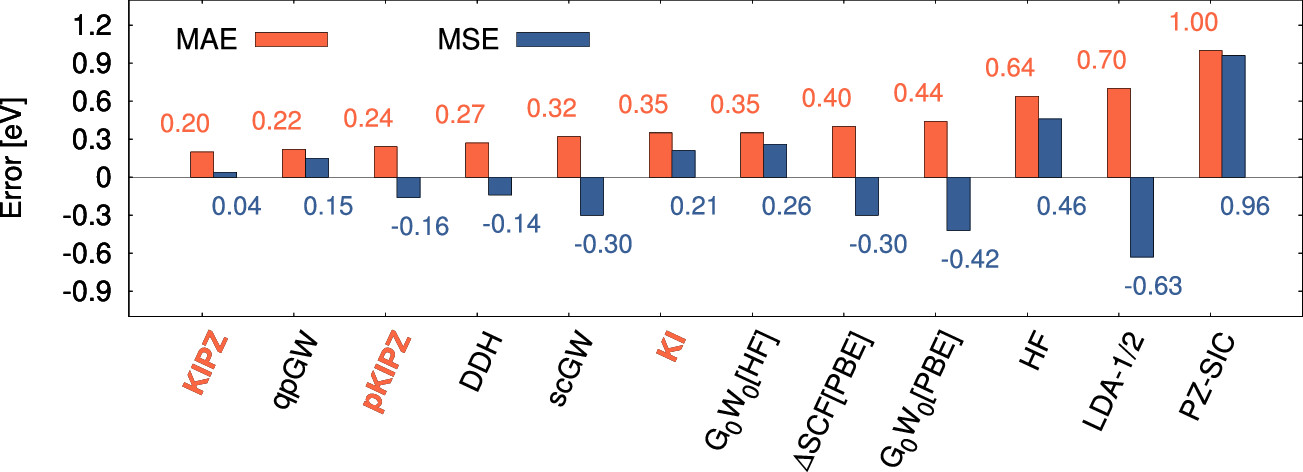
\includegraphics[width=\columnwidth]{figures/colonna_2019_gw100_ip.jpeg}
         \begin{center}
            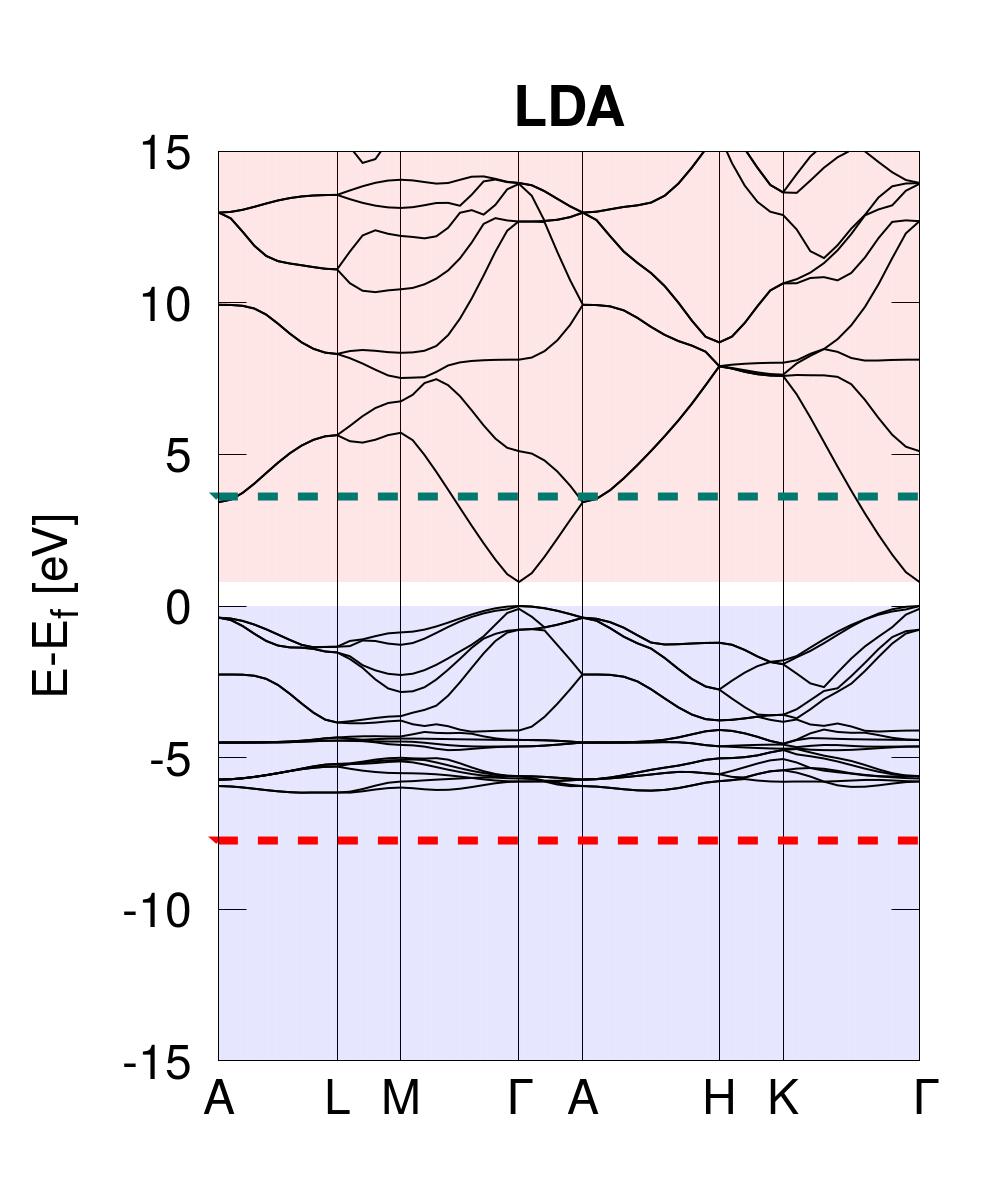
\includegraphics[width=0.45\columnwidth]{figures/ZnO_lda.png}
            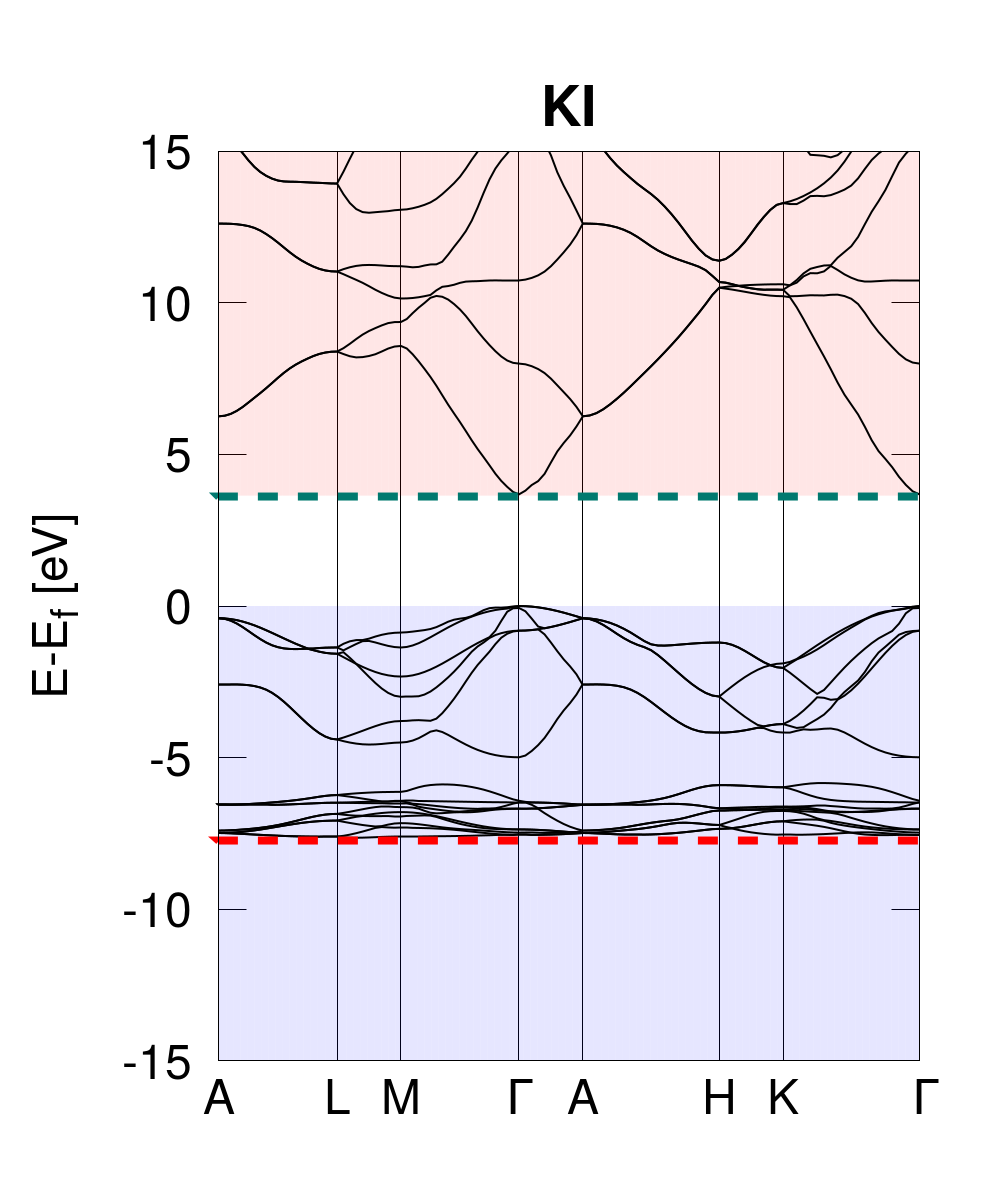
\includegraphics[width=0.45\columnwidth]{figures/ZnO_ki.png}
         \end{center}
      \end{column}
      \begin{column}{0.45\textwidth}
         \begin{itemize}
            \item orbital-density-dependent corrective terms to semi-local DFT
            \item comparable computational cost to DFPT
            \item KS eigenvalues are meaningful
            \item accuracy comparable to GW
         \end{itemize}

         caveats:
         \begin{itemize}
            \item orbital density dependence has limitations
            \item complicated workflow (not for much longer!)
            \item only for insulators
         \end{itemize}

      \end{column}
   \end{columns}

\end{frame}

\begin{frame}{Summary: thoughts on the way forward}
   For Koopmans...
   \begin{itemize}
      \item framing Koopmans with frozen-orbital/projector-like picture
      \item prediction of $\alpha_i$
      \item scope for addressing static correlation error
      \item off-diagonal terms
   \end{itemize}

   For corrections to SIE more generally\dots
   \begin{itemize}
      \item we can gain ground by thinking about KS energies and not just total energies
      \item indeed, KI corrects KS energies while leaving total energies untouched!
   \end{itemize}

\end{frame}

\begin{frame}{Acknowledgements}
   \begin{center}
      \footnotesize
      \begin{tabularx}{\textwidth}{CCCCCC}
         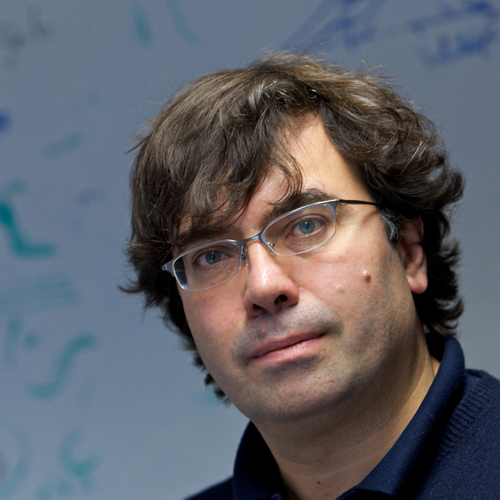
\includegraphics[height = 0.2\paperheight]{figures/nicola_marzari.jpg}   &
         
\includegraphics[height = 0.2\paperheight]{figures/nicola_colonna.png}   &
         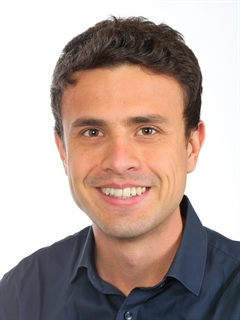
\includegraphics[height = 0.2\paperheight]{figures/yannick_schubert.jpg} &
         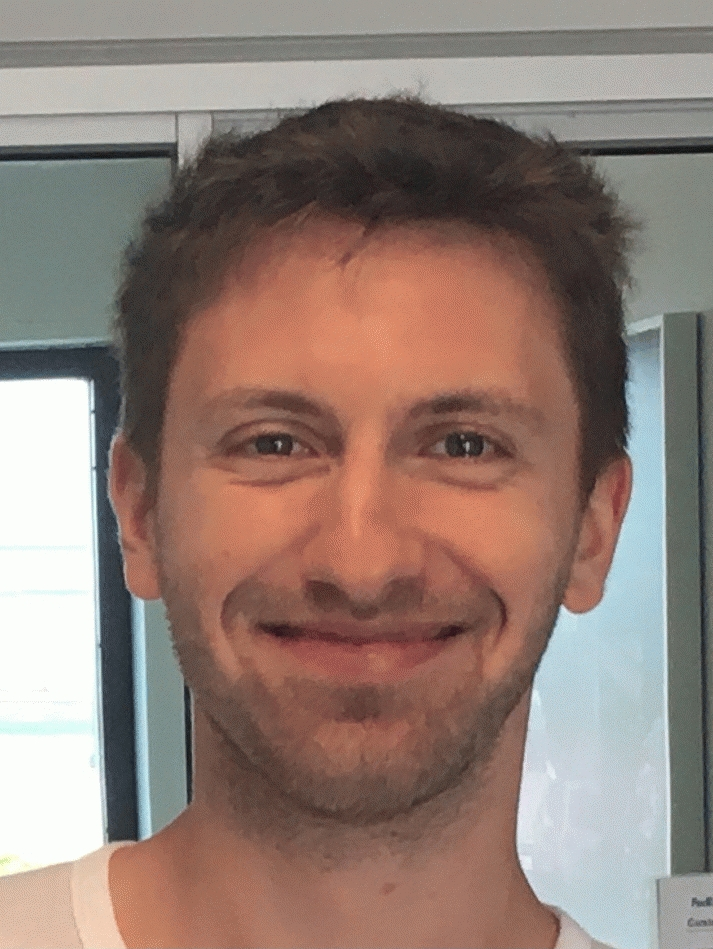
\includegraphics[height = 0.2\paperheight]{figures/riccardo_degennaro.jpg} \\
         % 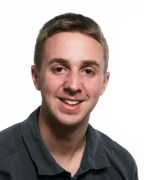
\includegraphics[height = 0.2\paperheight]{figures/daniel_cole.jpeg}       &
         % 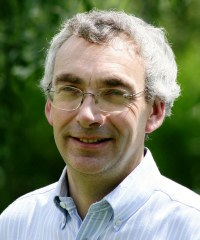
\includegraphics[height = 0.2\paperheight]{figures/mike_payne.jpeg}        &
         % 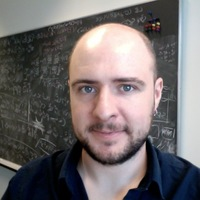
\includegraphics[height = 0.2\paperheight]{figures/david_oregan.jpg}         \\
         Nicola Marzari                                                           &
         Nicola Colonna                                                           &
         Riccardo De~Gennaro                                                      &
         Yannick Schubert                                                           \\
      \end{tabularx}
   \end{center}
   \begin{center}
      
\includegraphics[height = 0.1\paperheight]{figures/fig_snsf_logo.png}
      \hspace{1em}
      
\includegraphics[height = 0.1\paperheight]{figures/fig_EPSRC.jpg}
      \hspace{1em}
      
\includegraphics[height = 0.1\paperheight]{figures/fig_Rutherford_foundation.png}
      \hspace{1em}
      
\includegraphics[height = 0.1\paperheight]{figures/fig_CCEIT.jpeg}
   \end{center}
   % \begin{multicols}{2}
   %   \small
   %   \printbibliography
   %   \normalsize
   % \end{multicols}
   \vspace{2ex}
   Look out for our papers \& code release later this year (follow 
\includegraphics[height=\fontcharht\font`\B]{figures/Twitter_Bird.png} \textcolor{twitter_blue}{@ed\_linscott} for updates/get in touch for alpha access!)

   \textcolor{red}{Shameless postdoc/fellowship plug?}

   \scriptsize

   \setbeamercolor*{bibliography entry title}{fg=black}
   \setbeamercolor*{bibliography entry author}{fg=black}
   \setbeamercolor*{bibliography entry location}{fg=black}
   \setbeamercolor*{bibliography entry note}{fg=black}

   \vspace{2ex}
   \scriptsize
   For further reading on Koopmans functionals, see\cite{Dabo2010,Borghi2014,Nguyen2018,Colonna2018,Colonna2019}
\end{frame}


\end{document}
